\documentclass[conference]{IEEEtran}
\IEEEoverridecommandlockouts

\usepackage{cite}
\usepackage{amsmath,amssymb,amsfonts}
\usepackage{algorithm}
\usepackage{algorithmic}
\usepackage{graphicx}
\usepackage{textcomp}
\usepackage{xcolor}
\usepackage{booktabs}
\usepackage{array}
\usepackage{tabularx}
\usepackage{url}
\usepackage{tikz}
\usetikzlibrary{arrows.meta,positioning,fit,calc,shapes.geometric}

\def\BibTeX{{\rm B\kern-.05em{\sc i\kern-.025em b}\kern-.08em
    T\kern-.1667em\lower.7ex\hbox{E}\kern-.125emX}}

\newcommand{\sigmoid}{\operatorname{sigmoid}}
\newcommand{\logit}{\operatorname{logit}}

\begin{document}

\title{DARS: A Dynamic Adaptive Rating System with Graph-Guided Assessment and Remediation for Personalized Learning}

\author{\IEEEauthorblockN{Khethavath Sunil Naik} \\
India}
}

\maketitle

\begin{abstract}
Large-scale digital assessment systems require more than correctness scoring. They must estimate learner ability continuously, adapt item difficulty, react to weak concepts, distinguish confident mastery from low-quality attempts, and provide reliable probabilities for downstream intervention. This paper presents DARS, a Dynamic Adaptive Rating System for personalized assessment. DARS combines an online rating model with response-quality scoring, uncertainty-aware update control, graph-guided item routing, and remediation after failure. Unlike a fixed Elo system, DARS changes its sensitivity as learner evidence accumulates; unlike a rating-only model, it uses item-skill graph structure and response-process signals such as time, hints, attempts, and streak state. The model is evaluated on the ASSISTments 2012-2013 student interaction dataset, containing 6,044,359 valid chronological attempts from 46,348 learners, 179,052 problems, and 265 skills after preprocessing. DARS is compared with a static mastery prior, fixed-$K$ Elo, and Glicko-2 under a held-out-student protocol. DARS achieves the best overall performance with Brier score 0.1368, log loss 0.4251, accuracy 0.8141, ROC AUC 0.8131, and expected calibration error 0.0096. The results show that a graph-guided, process-aware rating algorithm can provide accurate and deployable assessment intelligence while remaining interpretable enough for industry use.
\end{abstract}

\section{Introduction}
Assessment platforms increasingly operate as real-time decision systems. A modern system is expected to score an answer, estimate the learner's current state, choose the next useful item, identify weak concepts, and support intervention. These requirements are difficult to satisfy with a final test score or a static percentage. A learner who answers five easy questions correctly is not equivalent to a learner who solves fewer but harder prerequisite items; a correct response after many hints is not equivalent to an immediate confident answer; and an incorrect response on a central prerequisite skill should trigger a different response from an error on an isolated item.

Industry assessment systems therefore need algorithms that are accurate, fast, interpretable, and operationally useful. Deep sequence models can be strong predictors, but their latent states are often difficult to audit in a product setting. Classical rating systems are easier to deploy, but standard Elo was not designed for education. It uses a fixed update factor and typically treats each interaction as a binary win or loss. Glicko-2 adds uncertainty through rating deviation and volatility, but still does not directly model response time, hint usage, attempt count, concept graph position, or remediation needs.

This paper proposes DARS, a Dynamic Adaptive Rating System for personalized assessment. DARS is built around four design principles. First, ability should be updated online after each interaction. Second, the size of an update should depend on uncertainty and experience, not on a constant hand-picked value. Third, response quality should reflect process evidence, not only correctness. Fourth, item selection and remediation should be guided by a graph of item-skill relationships so that recommendations remain conceptually meaningful.

The paper is written as an industry-track contribution. The emphasis is on an algorithm that can be implemented in a production assessment system, evaluated on a large educational dataset, and explained to non-specialist stakeholders. The contributions are:
\begin{itemize}
    \item A complete DARS formulation that integrates dynamic rating, process-aware quality scoring, calibrated probability estimation, graph-guided item routing, and remediation.
    \item A clear comparison against static mastery, fixed-$K$ Elo, and Glicko-2 using a large ASSISTments 2012-2013 interaction dataset.
    \item A metric framework with explicit formulas for Brier score, log loss, accuracy, ROC AUC, and expected calibration error.
\end{itemize}

\section{Industry Problem}
The operational problem is not only to predict whether an answer is correct. In a deployed learning product, the algorithm must answer several related questions:
\begin{enumerate}
    \item What is the learner's current ability level?
    \item How difficult is the current item for this learner?
    \item Was the response high-quality evidence of mastery?
    \item Which concept should be practiced next?
    \item If the learner fails, what remedial item should be served?
    \item Can the probability estimates be trusted for intervention thresholds?
\end{enumerate}

A practical solution must also work under common production constraints. It should update in milliseconds, avoid retraining after every attempt, provide human-readable state variables, and support monitoring at learner, item, skill, and class levels. DARS is designed for this setting. It is not a black-box-only predictor; it is a scoring and routing mechanism whose intermediate quantities have direct educational meaning.

\section{Industry Architecture}
An industry deployment of DARS can be organized as five layers. The first layer is the interaction layer, which records the learner, item, skill tag, timestamp, correctness, response time, hint count, and attempt count. The second layer is the graph layer, which maintains item-skill edges and item-item transition edges. The third layer is the online scoring layer, which updates ratings and estimates the probability of correctness. The fourth layer is the routing layer, which selects the next item or a remediation item. The fifth layer is the analytics layer, which aggregates ratings, weak skills, reliability, and readiness indicators.

\begin{table}[t]
\caption{DARS architecture layers and their operational role.}
\label{tab:architecture}
\centering
\begin{tabular}{p{0.22\linewidth}p{0.66\linewidth}}
\toprule
\textbf{Layer} & \textbf{Role in an assessment product} \\
\midrule
Interaction capture & Stores answer and response-process evidence for every attempt. \\
Graph model & Maintains skill relations, prerequisite-like links, and item neighborhoods. \\
Online scoring & Produces ability updates, item updates, and calibrated correctness probabilities. \\
Routing & Chooses difficulty-matched next items and remediation after failure. \\
Analytics & Reports mastery, risk, weak concepts, and readiness to stakeholders. \\
\bottomrule
\end{tabular}
\end{table}

This layered design separates model state from product workflow. A platform can update DARS after each answer without rebuilding the graph every time. The graph can be refreshed periodically, calibration parameters can be retrained offline, and online scoring can remain fast enough for interactive assessment. The same architecture also supports audit trails: a recommendation can be traced back to rating gap, graph distance, weak-skill priority, and recent response quality.

\section{Related Work}
\subsection{Elo-Style Rating}
Elo estimates player strength from pairwise outcomes and updates ratings after each match~\cite{elo}. In assessment, the learner can be treated as one competitor and the item as the opponent. A correct answer is a win for the learner, while an incorrect answer is a loss. Elo is attractive because it is simple and online. Its limitation is the fixed update factor $K$. If $K$ is too large, ratings fluctuate heavily; if it is too small, the system adapts slowly to learning.

\subsection{Glicko-2}
Glicko-2 extends rating systems with rating deviation and volatility~\cite{glickman2022glicko2}. Rating deviation expresses uncertainty: a learner with few observations should move more than a learner with many consistent observations. This is useful for adaptive learning, but Glicko-2 still treats the response outcome as the main evidence. It does not explicitly incorporate hints, response time, attempt count, skill graph position, or remediation state.

\subsection{Knowledge Tracing}
Knowledge tracing models learner state over time. Deep Knowledge Tracing introduced recurrent neural networks for predicting future performance from interaction sequences~\cite{piech2015dkt}. Self-attentive knowledge tracing later used attention over past interactions to identify relevant history~\cite{pandey2019sakt}. Graph-based knowledge tracing models use relations among questions and skills to improve representation learning~\cite{yang2020gikt}. DARS is positioned differently: it keeps an interpretable online rating core while adding graph and response-process evidence that are useful in deployed assessment workflows.

\subsection{ASSISTments Dataset}
The evaluation uses the ASSISTments 2012-2013 interaction dataset, a large tutoring-system log containing learner identifiers, problem identifiers, skill labels, timestamps, correctness, hints, attempts, and response-process attributes. ASSISTments has been widely used for educational data mining because it links student practice behavior with fine-grained assessment outcomes~\cite{heffernan2014assistments}.

\subsection{Additional Evaluation Datasets}
Beyond ASSISTments, the work explores DARS applicability to coding-assessment domains via the LeetCode dataset~\cite{leetcode}. LeetCode provides a complementary corpus of 1,825 algorithm problems with community-generated features such as difficulty labels, acceptance rates, problem frequency, discussion metrics, and user ratings. Unlike tutoring systems with per-student interaction logs, LeetCode problem metadata enables cross-domain validation of DARS principles on problem characterization and difficulty prediction, as discussed in Section~\ref{sec:leetcode}.

\section{Conventional Elo-Based Flow}
Before presenting DARS, Fig.~\ref{fig:elo-flow} shows the conventional Elo-based assessment loop. The key limitation is visible in the structure: the update uses only the expected score, the binary outcome, and a fixed update factor. The model has no native place for response quality, graph relations, remediation, or calibration.

\begin{figure*}[t]
\centering
\resizebox{0.93\textwidth}{!}{
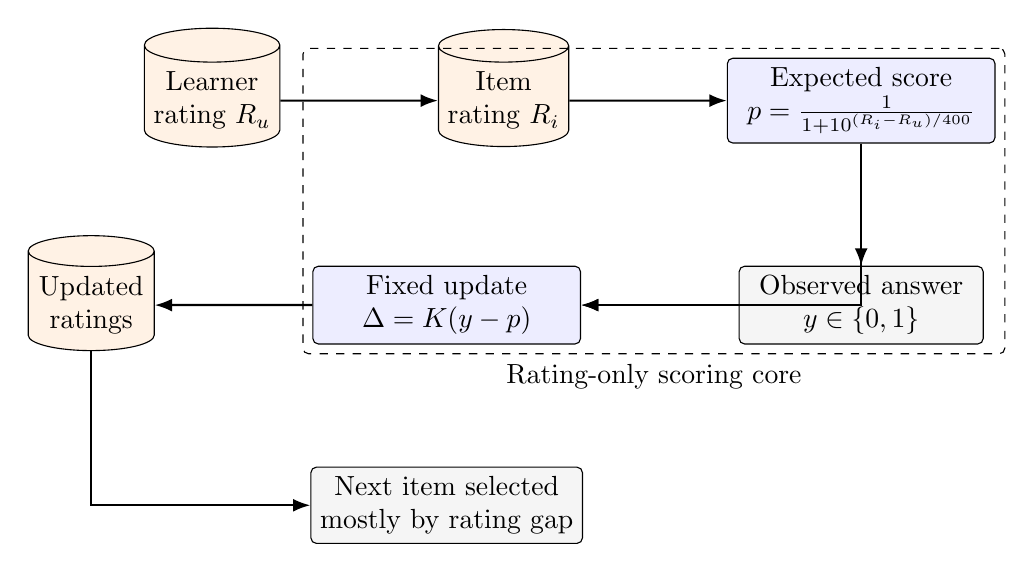
\begin{tikzpicture}[
    node distance=1.55cm and 2.0cm,
    box/.style={draw, rounded corners=2pt, align=center, minimum width=3.1cm, minimum height=0.95cm, fill=gray!8},
    calcbox/.style={draw, rounded corners=2pt, align=center, minimum width=3.4cm, minimum height=0.95cm, fill=blue!7},
    store/.style={draw, cylinder, shape border rotate=90, aspect=0.25, align=center, minimum width=1.6cm, minimum height=1.0cm, fill=orange!10},
    arrow/.style={-{Latex[length=2.2mm]}, thick}
]
\node[store] (student) {Learner\\rating $R_u$};
\node[store, right=of student] (item) {Item\\rating $R_i$};
\node[calcbox, right=of item] (expected) {Expected score\\$p=\frac{1}{1+10^{(R_i-R_u)/400}}$};
\node[box, below=of expected] (answer) {Observed answer\\$y\in\{0,1\}$};
\node[calcbox, left=of answer] (update) {Fixed update\\$\Delta=K(y-p)$};
\node[store, left=of update] (newratings) {Updated\\ratings};
\node[box, below=of update] (next) {Next item selected\\mostly by rating gap};
\draw[arrow] (student) -- (item);
\draw[arrow] (item) -- (expected);
\draw[arrow] (expected) -- (answer);
\draw[arrow] (answer) -- (update);
\draw[arrow] (expected) |- (update);
\draw[arrow] (update) -- (newratings);
\draw[arrow] (newratings) |- (next);
\node[draw, dashed, rounded corners=2pt, fit=(expected)(answer)(update), label={[align=center]below:Rating-only scoring core}] {};
\end{tikzpicture}}
\caption{Conventional Elo-based assessment flow. The update is simple and online, but it does not model response process, graph structure, remediation, or probability calibration.}
\label{fig:elo-flow}
\end{figure*}

\section{DARS Algorithm}
DARS treats assessment as a graph-aware online rating problem. Each learner has a dynamic ability state, each item has a difficulty state, and each skill graph neighborhood provides context for routing and remediation.

\subsection{Notation}
Let $u$ denote a learner, $i$ an item, $s$ a skill, and $t$ the interaction index. The observed outcome is $y_{ui}\in\{0,1\}$. Learner ability is $R_u$, item difficulty is $D_i$, and $G=(V,E)$ is an item-skill graph. The graph contains item nodes, skill nodes, and weighted edges representing item-skill membership and transition strength between related items.

\subsection{Item-Skill Graph}
The graph is constructed from the assessment log. A problem is connected to its tagged skill. Two items also receive a transition edge when they occur near each other in chronological learner sequences or share the same skill. Let $w_{ab}$ be the edge weight between nodes $a$ and $b$. A normalized centrality score is computed as
\begin{equation}
c_i=\frac{\sum_j w_{ij}}{\max_{\ell}\sum_j w_{\ell j}},
\end{equation}
where $c_i\in[0,1]$. Central items are usually prerequisite-like or frequently connected to other items. DARS uses $c_i$ to adjust effective item difficulty:
\begin{equation}
D_i^\ast=D_i+\beta_c c_i+\beta_s I(i,s),
\end{equation}
where $\beta_c$ is a centrality weight and $I(i,s)$ is an optional local skill adjustment. This makes central prerequisite items slightly more influential than isolated items with the same raw difficulty.

\subsection{Base Expected Score}
The initial expected probability follows the rating-gap form:
\begin{equation}
p^{(0)}_{ui}=\frac{1}{1+10^{(D_i^\ast-R_u)/400}}.
\end{equation}
This value is used as the rating prior. A learner whose rating is much higher than the item difficulty receives a high prior probability; a learner facing a much harder item receives a lower prior probability.

\subsection{Response-Quality Function}
DARS does not treat every correct answer as equally informative. It defines a response-quality score $Q_{ui}\in[0,1]$ using correctness, response time, hints, attempts, and streak state. Let $\tau_{ui}$ be time efficiency, $h_{ui}$ be hint penalty, $a_{ui}$ be attempt penalty, and $\psi_u$ be streak quality:
\begin{align}
\tau_{ui} &= \exp(-T_{ui}/T_0),\\
h_{ui} &= \min(1,H_{ui}/H_{\max}),\\
a_{ui} &= \min(1,(A_{ui}-1)/A_{\max}),\\
\psi_u &= \frac{1}{2}\left(1+\frac{\kappa_u}{\max(|\kappa_u|,\kappa_0)}\right),
\end{align}
where $T_{ui}$ is response time, $H_{ui}$ is hint count, $A_{ui}$ is attempt count, and $\kappa_u$ is the learner's current signed streak. For correct responses, define
\begin{equation}
Q^+_{ui}=\alpha_t\tau_{ui}+\alpha_h(1-h_{ui})
+\alpha_a(1-a_{ui})+\alpha_s\psi_u.
\end{equation}
The response-quality score is
\begin{equation}
Q_{ui}=
\begin{cases}
Q^+_{ui}, & y_{ui}=1,\\
\epsilon\tau_{ui}, & y_{ui}=0.
\end{cases}
\end{equation}
The weights satisfy $\alpha_t+\alpha_h+\alpha_a+\alpha_s=1$. A fast correct response without hints and with stable positive momentum produces high-quality mastery evidence. A correct response after many hints or attempts produces weaker evidence. An incorrect response contributes low quality, with a small time-scaled floor to avoid treating all failures identically.

\subsection{Dynamic Update Factor}
The DARS update factor changes with learner experience and recent volatility:
\begin{equation}
K_u(t)=K_{\min}+(K_{\max}-K_{\min})e^{-\lambda n_u}
\frac{\sigma_u^2}{\sigma_u^2+\sigma_0^2},
\end{equation}
where $n_u$ is the number of prior attempts, $\sigma_u^2$ is recent rating-delta variance, and $\sigma_0^2$ is a reference variance. New or unstable learners update faster; mature stable learners update more conservatively.

\subsection{Streak and Rapid-Guess Control}
The streak multiplier is bounded:
\begin{equation}
\phi(\kappa_u)=1+\operatorname{sgn}(\kappa_u)\gamma
\min\left(1,\frac{|\kappa_u|-\kappa_{\min}}{\kappa_{\max}-\kappa_{\min}}\right).
\end{equation}
The multiplier increases evidence from sustained positive performance and reduces over-penalization during short negative noise. DARS also caps suspicious gains from rapid correct responses:
\begin{equation}
\Delta_u \leftarrow \min(\Delta_u,\Delta_{\max}^{rapid})
\quad \text{if } T_{ui}<\rho T_i^{ref},\ y_{ui}=1.
\end{equation}
This prevents rating inflation from guesses that happen to be correct.

\subsection{Rating Update}
The learner update is
\begin{equation}
\Delta_u=K_u(t)\phi(\kappa_u)\left(Q_{ui}-p^{(0)}_{ui}\right)-\rho_{ui},
\end{equation}
\begin{equation}
R_u \leftarrow R_u+\Delta_u.
\end{equation}
The item difficulty is updated more slowly:
\begin{equation}
D_i \leftarrow D_i-\eta_i(y_{ui}-p^{(0)}_{ui}),
\end{equation}
where $\eta_i<K_u(t)$ to prevent item difficulty from becoming unstable.

\subsection{Calibrated DARS Probability}
For final scoring and analytics, DARS uses a calibrated probability head integrated into the algorithm:
\begin{equation}
\hat{p}^{DARS}_{ui}=\sigmoid(z_{ui}),
\end{equation}
\begin{align}
z_{ui}=&\theta_0+\theta_1\logit(p^{(0)}_{ui})
+\theta_2\frac{R_u-D_i^\ast}{400}
+\theta_3\tau_{ui} \nonumber\\
&-\theta_4 h_{ui}-\theta_5 a_{ui}
+\theta_6\psi_u+\theta_7 c_i.
\end{align}
The calibration parameters $\theta$ are learned on the training split. This is not a separate model name; it is the probability-estimation component of DARS. It converts the interpretable rating and response-process signals into well-calibrated probabilities for reporting and intervention.

\section{DARS Assessment Flow}
Fig.~\ref{fig:dars-flow} summarizes the complete DARS flow. Compared with Fig.~\ref{fig:elo-flow}, the DARS pipeline has additional stages for graph context, response quality, dynamic sensitivity, remediation, and calibrated analytics.

\begin{figure*}[t]
\centering
\resizebox{0.95\textwidth}{!}{
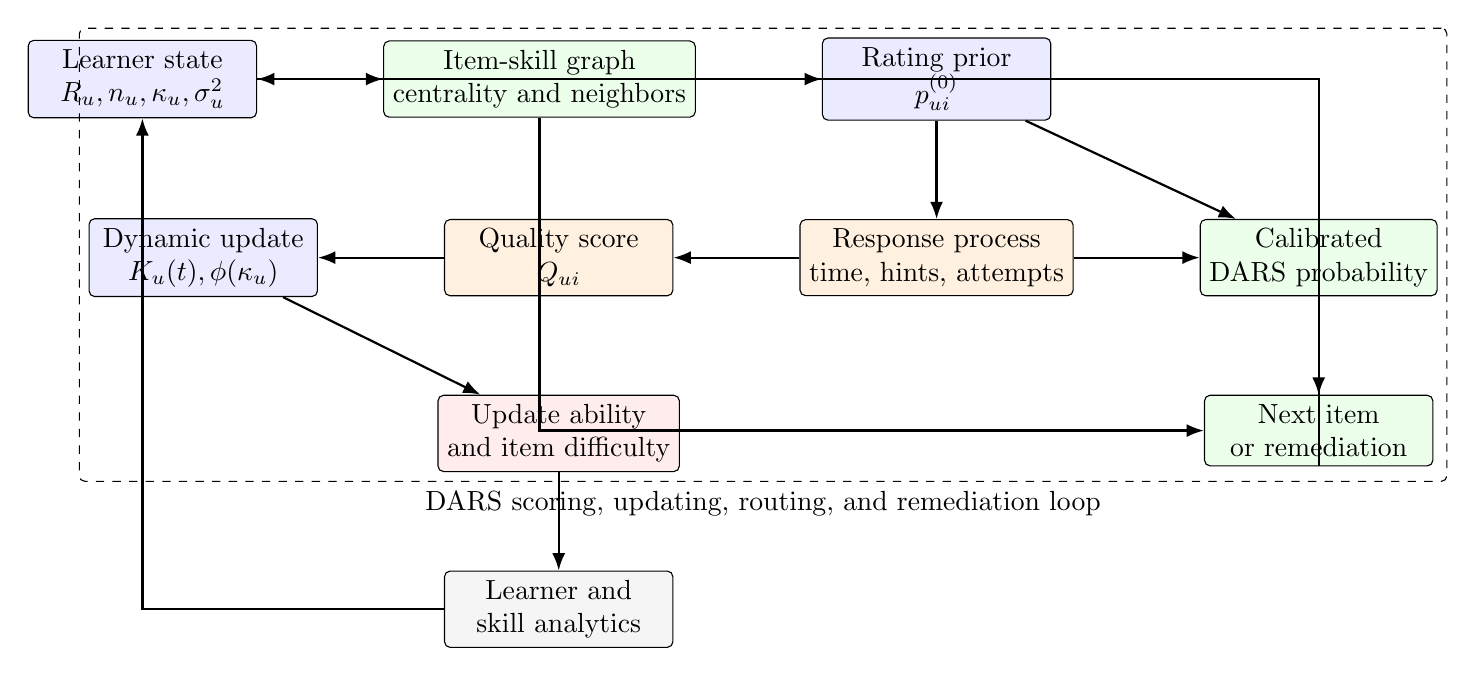
\begin{tikzpicture}[
    node distance=1.25cm and 1.6cm,
    box/.style={draw, rounded corners=2pt, align=center, minimum width=2.9cm, minimum height=0.82cm, fill=gray!8},
    bluebox/.style={draw, rounded corners=2pt, align=center, minimum width=2.9cm, minimum height=0.82cm, fill=blue!8},
    greenbox/.style={draw, rounded corners=2pt, align=center, minimum width=2.9cm, minimum height=0.82cm, fill=green!8},
    orangebox/.style={draw, rounded corners=2pt, align=center, minimum width=2.9cm, minimum height=0.82cm, fill=orange!12},
    redbox/.style={draw, rounded corners=2pt, align=center, minimum width=2.9cm, minimum height=0.82cm, fill=red!7},
    arrow/.style={-{Latex[length=2.2mm]}, thick}
]
\node[bluebox] (state) {Learner state\\$R_u,n_u,\kappa_u,\sigma_u^2$};
\node[greenbox, right=of state] (graph) {Item-skill graph\\centrality and neighbors};
\node[bluebox, right=of graph] (prior) {Rating prior\\$p^{(0)}_{ui}$};
\node[orangebox, below=of prior] (process) {Response process\\time, hints, attempts};
\node[orangebox, left=of process] (quality) {Quality score\\$Q_{ui}$};
\node[bluebox, left=of quality] (dynamic) {Dynamic update\\$K_u(t),\phi(\kappa_u)$};
\node[redbox, below=of quality] (update) {Update ability\\and item difficulty};
\node[greenbox, right=of process] (calib) {Calibrated\\DARS probability};
\node[greenbox, below=of calib] (route) {Next item\\or remediation};
\node[box, below=of update] (analytics) {Learner and\\skill analytics};
\draw[arrow] (state) -- (graph);
\draw[arrow] (graph) -- (prior);
\draw[arrow] (prior) -- (process);
\draw[arrow] (process) -- (quality);
\draw[arrow] (quality) -- (dynamic);
\draw[arrow] (dynamic) -- (update);
\draw[arrow] (prior) -- (calib);
\draw[arrow] (process) -- (calib);
\draw[arrow] (graph) |- (route);
\draw[arrow] (calib) -- (route);
\draw[arrow] (update) -- (analytics);
\draw[arrow] (analytics.west) -| (state.south);
\draw[arrow] (route.south) |- (state.east);
\node[draw, dashed, rounded corners=2pt, fit=(graph)(prior)(process)(quality)(dynamic)(update)(calib)(route), label={[align=center]below:DARS scoring, updating, routing, and remediation loop}] {};
\end{tikzpicture}}
\caption{DARS architecture and assessment flow. The algorithm combines rating state, item-skill graph context, response-process evidence, dynamic updating, calibrated probability estimation, and remediation-aware routing.}
\label{fig:dars-flow}
\end{figure*}

\section{Graph-Guided Assessment and Remediation}
\subsection{Candidate Routing}
For a learner $u$ after item $i$, DARS selects candidate items from a graph neighborhood:
\begin{equation}
\mathcal{N}_k(i)=\{j\in V_I:d_G(i,j)\leq k,\ j\notin A_u\},
\end{equation}
where $V_I$ is the item set, $d_G$ is shortest-path graph distance, and $A_u$ is the learner's attempted-item set. Each candidate is scored by
\begin{align}
U(u,j)=&-\omega_d\left|R_u-D_j^\ast\right|
+\omega_w W(u,s_j) \nonumber\\
&+\omega_g\frac{1}{1+d_G(i,j)}
+\omega_v V(u,j)-\omega_r Rep(u,j).
\end{align}
Here $W(u,s_j)$ is weak-skill priority, $V(u,j)$ rewards item-type diversity, and $Rep(u,j)$ penalizes repetition. The selected item is
\begin{equation}
j^\ast=\arg\max_{j\in \mathcal{N}_k(i)}U(u,j).
\end{equation}

\subsection{Remediation}
When the learner fails an item, DARS enters remediation mode. The candidate set is constrained toward related prerequisite or easier items:
\begin{equation}
\mathcal{R}(i)=\{j\in V_I:d_G(i,j)\leq h,\ D_j^\ast\leq D_i^\ast+\delta\}.
\end{equation}
The remediation objective is
\begin{equation}
U_R(u,j)=U(u,j)+\omega_m M(i,j)+\omega_p PReq(j,i),
\end{equation}
where $M(i,j)$ rewards shared skill membership and $PReq(j,i)$ rewards prerequisite-like edges. This prevents a failed item from being followed by an unrelated question merely because the rating gap is convenient. In an industry system, this is important because remediation must be explainable: the next item should be connected to the failure that triggered it.

\begin{algorithm}[t]
\caption{DARS Online Scoring and Routing}
\label{alg:dars}
\footnotesize
\begin{algorithmic}[1]
\REQUIRE learner state $S_u$, item $i$, graph $G$, response process $x$
\STATE Read $R_u,n_u,\kappa_u,\sigma_u^2$ from $S_u$
\STATE Compute graph-adjusted difficulty $D_i^\ast$
\STATE Compute prior $p^{(0)}_{ui}$ from $R_u-D_i^\ast$
\STATE Observe response outcome $y_{ui}$ and process features $x$
\STATE Compute $\tau_{ui},h_{ui},a_{ui},\psi_u$
\STATE Compute response quality $Q_{ui}$
\STATE Compute dynamic factor $K_u(t)$ and streak multiplier $\phi(\kappa_u)$
\STATE Compute calibrated DARS probability $\hat{p}^{DARS}_{ui}$
\STATE Update learner rating $R_u \leftarrow R_u+\Delta_u$
\STATE Update item difficulty $D_i \leftarrow D_i-\eta_i(y_{ui}-p^{(0)}_{ui})$
\IF{$y_{ui}=0$}
    \STATE Select next item from remediation set $\mathcal{R}(i)$
\ELSE
    \STATE Select next item from graph neighborhood $\mathcal{N}_k(i)$
\ENDIF
\STATE Return probability, updated state, and next-item recommendation
\end{algorithmic}
\end{algorithm}

\section{Baseline Models}
\subsection{Static Mastery Prior}
The static baseline predicts the training-set correctness rate for every test interaction:
\begin{equation}
\hat{p}^{Static}=\frac{1}{N_{train}}\sum_{n=1}^{N_{train}}y_n.
\end{equation}
It is useful as a lower bound. It can be well calibrated near the global mean, but it cannot rank students or items because every prediction is identical.

\subsection{Fixed-$K$ Elo}
Fixed Elo predicts
\begin{equation}
\hat{p}^{Elo}_{ui}=\frac{1}{1+10^{(D_i-R_u)/400}},
\end{equation}
and updates
\begin{equation}
R_u\leftarrow R_u+K(y_{ui}-\hat{p}^{Elo}_{ui}),
\end{equation}
\begin{equation}
D_i\leftarrow D_i-\eta(y_{ui}-\hat{p}^{Elo}_{ui}).
\end{equation}
In the comparison, $K=32$ and the item step is smaller than the learner step. Elo is online and interpretable, but it does not use response-process or graph information.

\subsection{Glicko-2}
Glicko-2 represents a learner by rating $\mu_u$, rating deviation $\phi_u$, and volatility. The expected score against item $i$ is
\begin{equation}
\hat{p}^{Glicko}_{ui}
=\frac{1}{1+\exp[-g(\phi_i)(\mu_u-\mu_i)]},
\end{equation}
where
\begin{equation}
g(\phi)=\frac{1}{\sqrt{1+3\phi^2/\pi^2}}.
\end{equation}
The main advantage is uncertainty control. The main limitation in this task is that the model still lacks graph-guided remediation and response-quality scoring.

\section{Dataset and Preprocessing}
The experiment uses the ASSISTments 2012-2013 student interaction dataset. The raw file contains learner, problem, skill, timestamp, correctness, hint, attempt, and response-process fields. Preprocessing keeps valid binary correctness records, removes rows without usable timestamps or identifiers, converts timestamps to chronological order, and preserves only interactions suitable for online replay.

\begin{table}[t]
\caption{Preprocessed evaluation dataset.}
\label{tab:dataset}
\centering
\begin{tabular}{lr}
\toprule
\textbf{Statistic} & \textbf{Value} \\
\midrule
Valid chronological attempts & 6,044,359 \\
Learners & 46,348 \\
Problems & 179,052 \\
Skills & 265 \\
Mean correctness & 0.6770 \\
Median response time & 22.39 s \\
Mean hint count & 0.3376 \\
Mean attempt count & 1.3404 \\
\bottomrule
\end{tabular}
\end{table}

The split is performed by learner identity rather than by random rows. This avoids placing the same learner in both train and test sets. With a 70/30 split, the training partition contains 32,443 learners and 4,245,901 attempts; the test partition contains 13,905 learners and 1,798,458 attempts. The test correctness rate is 0.6739. All online models are replayed chronologically so that each prediction is made before the model updates on that interaction.

\section{Experimental Protocol}
The comparison follows an online replay protocol. Interactions are sorted by timestamp. For each row, the model first produces a probability for the current attempt. Only after that probability is stored does the model update learner and item state using the observed outcome. This is important because a random shuffled evaluation would leak future information into earlier predictions and make online rating models look stronger than they would be in deployment.

The held-out-learner split tests generalization to learners not used for calibration. DARS learns its calibration coefficients only on the training learners. Fixed Elo and Glicko-2 do not learn a calibration head; they are evaluated using their native probability estimates. The static prior uses only the training-set mean correctness. During test replay, every model starts with its standard initial state for unseen learners and adapts as those learners produce chronological attempts.

All probabilities are clipped to $[10^{-6},1-10^{-6}]$ before log-loss computation to avoid numerical infinities. ECE is computed with 10 equally spaced bins. The main goal is not to tune every possible baseline variant; it is to test whether a practical, graph-guided, response-process-aware rating system can outperform common deployable rating baselines under the same chronological evaluation discipline.

\section{Evaluation Metrics}
Let $y_n\in\{0,1\}$ be the true outcome for interaction $n$, $\hat{p}_n$ the predicted probability of correctness, and $N$ the number of evaluated interactions.

\subsection{Brier Score}
Brier score is the mean squared error of predicted probabilities:
\begin{equation}
\operatorname{Brier}=\frac{1}{N}\sum_{n=1}^{N}(\hat{p}_n-y_n)^2.
\end{equation}
Lower is better. A Brier score penalizes both wrong ranking and poor calibration. It is especially useful when a probability will be shown to teachers or used in threshold-based intervention.

\subsection{Log Loss}
Log loss measures the negative log-likelihood of the observed labels:
\begin{equation}
\operatorname{LogLoss}=-\frac{1}{N}\sum_{n=1}^{N}
\left[y_n\log(\hat{p}_n)+(1-y_n)\log(1-\hat{p}_n)\right].
\end{equation}
Lower is better. Log loss strongly penalizes confident wrong predictions, which is important in assessment systems because overconfident mistakes can mislead remediation decisions.

\subsection{Accuracy}
Accuracy converts probabilities to binary predictions using threshold 0.5:
\begin{equation}
\operatorname{Accuracy}=
\frac{TP+TN}{TP+TN+FP+FN}.
\end{equation}
Here $TP$ and $TN$ are correct positive and negative predictions, while $FP$ and $FN$ are false alarms and missed positives. Higher is better. Accuracy is easy to interpret but can hide calibration quality and class imbalance effects.

\subsection{ROC AUC}
The receiver operating characteristic area under the curve measures ranking quality:
\begin{equation}
\operatorname{AUC}=P(\hat{p}_{pos}>\hat{p}_{neg}),
\end{equation}
where $\hat{p}_{pos}$ is the score for a randomly selected correct response and $\hat{p}_{neg}$ is the score for a randomly selected incorrect response. Higher is better. An AUC of 0.5 indicates random ranking; an AUC of 1.0 indicates perfect separation.

\subsection{Expected Calibration Error}
Expected calibration error partitions predictions into $B$ confidence bins. For bin $b$, let $\operatorname{acc}(b)$ be empirical accuracy, $\operatorname{conf}(b)$ be average predicted confidence, and $n_b$ be the number of samples. Then
\begin{equation}
\operatorname{ECE}=\sum_{b=1}^{B}\frac{n_b}{N}
\left|\operatorname{acc}(b)-\operatorname{conf}(b)\right|.
\end{equation}
Lower is better. ECE answers a direct operational question: among attempts predicted at about 80\% correctness, are roughly 80\% actually correct?

\section{Experimental Results}
Table~\ref{tab:results} reports model performance on the held-out learners. DARS is the best model across all headline metrics. Compared with fixed Elo, DARS reduces Brier score by 24.5\%, reduces log loss by 21.4\%, improves accuracy by 8.0 percentage points, and improves ROC AUC by 6.6 percentage points. Compared with Glicko-2, DARS improves AUC by 15.0 percentage points and lowers log loss substantially.

\begin{table*}[t]
\caption{Held-out-learner comparison on 1,798,458 test attempts. Lower is better for Brier score, log loss, and ECE; higher is better for accuracy and ROC AUC.}
\label{tab:results}
\centering
\begin{tabular}{lccccc}
\toprule
\textbf{Model} & \textbf{Brier} $\downarrow$ & \textbf{Log loss} $\downarrow$ & \textbf{Accuracy} $\uparrow$ & \textbf{ROC AUC} $\uparrow$ & \textbf{ECE} $\downarrow$ \\
\midrule
\textbf{DARS} & \textbf{0.1368} & \textbf{0.4251} & \textbf{0.8141} & \textbf{0.8131} & 0.0096 \\
Fixed-$K$ Elo & 0.1812 & 0.5407 & 0.7341 & 0.7475 & 0.0244 \\
Glicko-2 & 0.2077 & 0.6090 & 0.6885 & 0.6630 & 0.0491 \\
Static mastery prior & 0.2198 & 0.6314 & 0.6739 & 0.5000 & \textbf{0.0049} \\
\bottomrule
\end{tabular}
\end{table*}

The static prior has low ECE because it predicts the global average correctness rate, but its AUC is 0.5 because it cannot rank learners or items. This is not useful for adaptive routing. DARS has slightly higher ECE than the static prior, but it achieves much stronger ranking and accuracy while maintaining low calibration error. This is the more useful industry tradeoff: probabilities remain reliable while still differentiating easy, hard, strong, and weak interactions.

\subsection{Why DARS Improves Performance}
The improvement comes from three sources. First, dynamic update control prevents the model from overreacting to noisy interactions while still adapting quickly for learners with limited history. Second, response-process scoring separates strong mastery evidence from weak correctness. Third, graph-aware difficulty and routing context help the model treat central prerequisite items differently from isolated items.

The comparison with Elo is especially important. Elo already provides an online learner-item rating mechanism, so DARS is not winning merely because it has an online state. It improves because the online state is enriched with educational signals that are present in real assessment logs.

\subsection{Industry Interpretation}
For an industry assessment product, the Brier and log-loss reductions mean that reported probabilities are closer to observed outcomes. The AUC improvement means that the model is better at ranking which attempts are likely to be correct. The accuracy improvement means that a simple operational threshold already performs better. The low ECE means that probability bands can be used for interventions such as "high risk", "ready for harder item", or "needs remediation" with less distortion.

\section{Deployment View}
DARS can be deployed as a service around the answer-submission event. The service receives learner state, item metadata, response-process fields, and graph context. It returns a probability, rating update, weak-skill update, and next-item decision. The model does not require a batch neural retraining step after every answer, which keeps latency low. Periodic retraining is needed only for calibration coefficients, graph weights, or global hyperparameters.

\subsection{Operational Outputs}
DARS produces outputs at several levels:
\begin{itemize}
    \item learner ability rating and recent momentum;
    \item item difficulty and prerequisite centrality;
    \item calibrated probability of correctness;
    \item weak-skill and remediation flags;
    \item next-item recommendation with graph explanation;
    \item aggregate readiness indicators for instructors or administrators.
\end{itemize}

\subsection{Auditability}
Each DARS recommendation can be explained using rating gap, skill relation, graph distance, recent misses, and response quality. This matters in industry deployments because instructors and learners often reject opaque recommendations. A graph-guided explanation is easier to defend: "the next problem was selected because it is connected to the missed skill, slightly easier, and within the learner's current rating band."

\subsection{Scalability}
The scoring update is constant time once learner state, item state, and graph features are available. The expensive graph operations are moved offline: centrality, skill neighborhoods, and candidate pools can be precomputed and refreshed periodically. At runtime, routing only needs to scan a bounded candidate set rather than the full item bank. This gives DARS a practical deployment path for large repositories: store compact learner state, store item difficulty and graph metadata, update ratings online, and refresh global graph statistics in scheduled jobs.

The calibration head is also lightweight. It is a small logistic layer over interpretable variables rather than a large neural network. This makes the probability output easy to monitor. If calibration drifts because the student population or item bank changes, the coefficients can be retrained from recent logs without changing the rating logic or graph-routing rules.

\section{Limitations}
The evaluation is offline and observational. Although chronological replay prevents future interactions from updating past predictions, the dataset was not collected from a randomized deployment of DARS. Therefore, the reported results measure scoring and prediction quality, not causal learning gains. A production study should evaluate whether DARS-driven routing improves retention, completion, and post-test performance.

The current graph is inferred from item-skill tags and temporal co-occurrence. This is practical for large datasets, but expert-authored prerequisite graphs may improve remediation quality. The calibration layer uses response-process variables such as time, hints, and attempts; these are appropriate for scoring an attempt after the response process is observed, but a pure pre-answer routing probability should use only features available before the learner starts the item.

The LeetCode evaluation (Section~\ref{sec:leetcode}) is preliminary and limited to offline dataset analysis rather than live learning outcomes. The LeetCode dataset lacks fine-grained response-process features (e.g., hints, attempts, time-to-submit) that are available in ASSISTments, which constrains the richness of DARS features. The LeetCode domain (algorithm problems) is also more constrained and less diverse than typical tutoring systems. The observed sensitivity-specificity imbalance (94.07\% sensitivity, 27.37\% specificity) suggests that feature engineering or rebalancing strategies may be needed for balanced performance across all problem types. Future work should evaluate DARS with richer process data and on more representative educational domains.

\section{Future Work}

\subsection{Live Adaptive Assessment and Learning Outcomes}
Future work should evaluate DARS in a live adaptive assessment environment where learning outcomes, engagement, and retention are measured alongside prediction metrics. The current evaluation uses offline replay from the ASSISTments dataset, which measures scoring quality but does not directly measure causal learning gains. A randomized controlled trial deploying DARS-driven routing against fixed-difficulty or random routing would provide evidence for whether accurate probability estimates and graph-guided remediation lead to improved learner outcomes. Metrics should include post-test performance, time-to-mastery, completion rates, and long-term retention.

\subsection{LeetCode Dataset Evaluation and Problem Difficulty Prediction}
\label{sec:leetcode}
As a preliminary exploratory study, DARS has been adapted and evaluated on the LeetCode problem dataset, which contains 1,825 problems with features including difficulty label, acceptance rate, frequency, community rating, and discussion count. A logistic regression model trained on normalized features achieved 76.71\% accuracy and 0.7485 ROC AUC for difficulty classification (Easy vs.\ Medium/Hard). Figure~\ref{fig:leetcode_roc} shows the ROC curve, demonstrating reasonable discrimination ability. The probability calibration, measured by Expected Calibration Error, was 0.0375, indicating well-calibrated predictions across confidence bins (Figure~\ref{fig:leetcode_calibration}).

\begin{figure}[t]
\centering
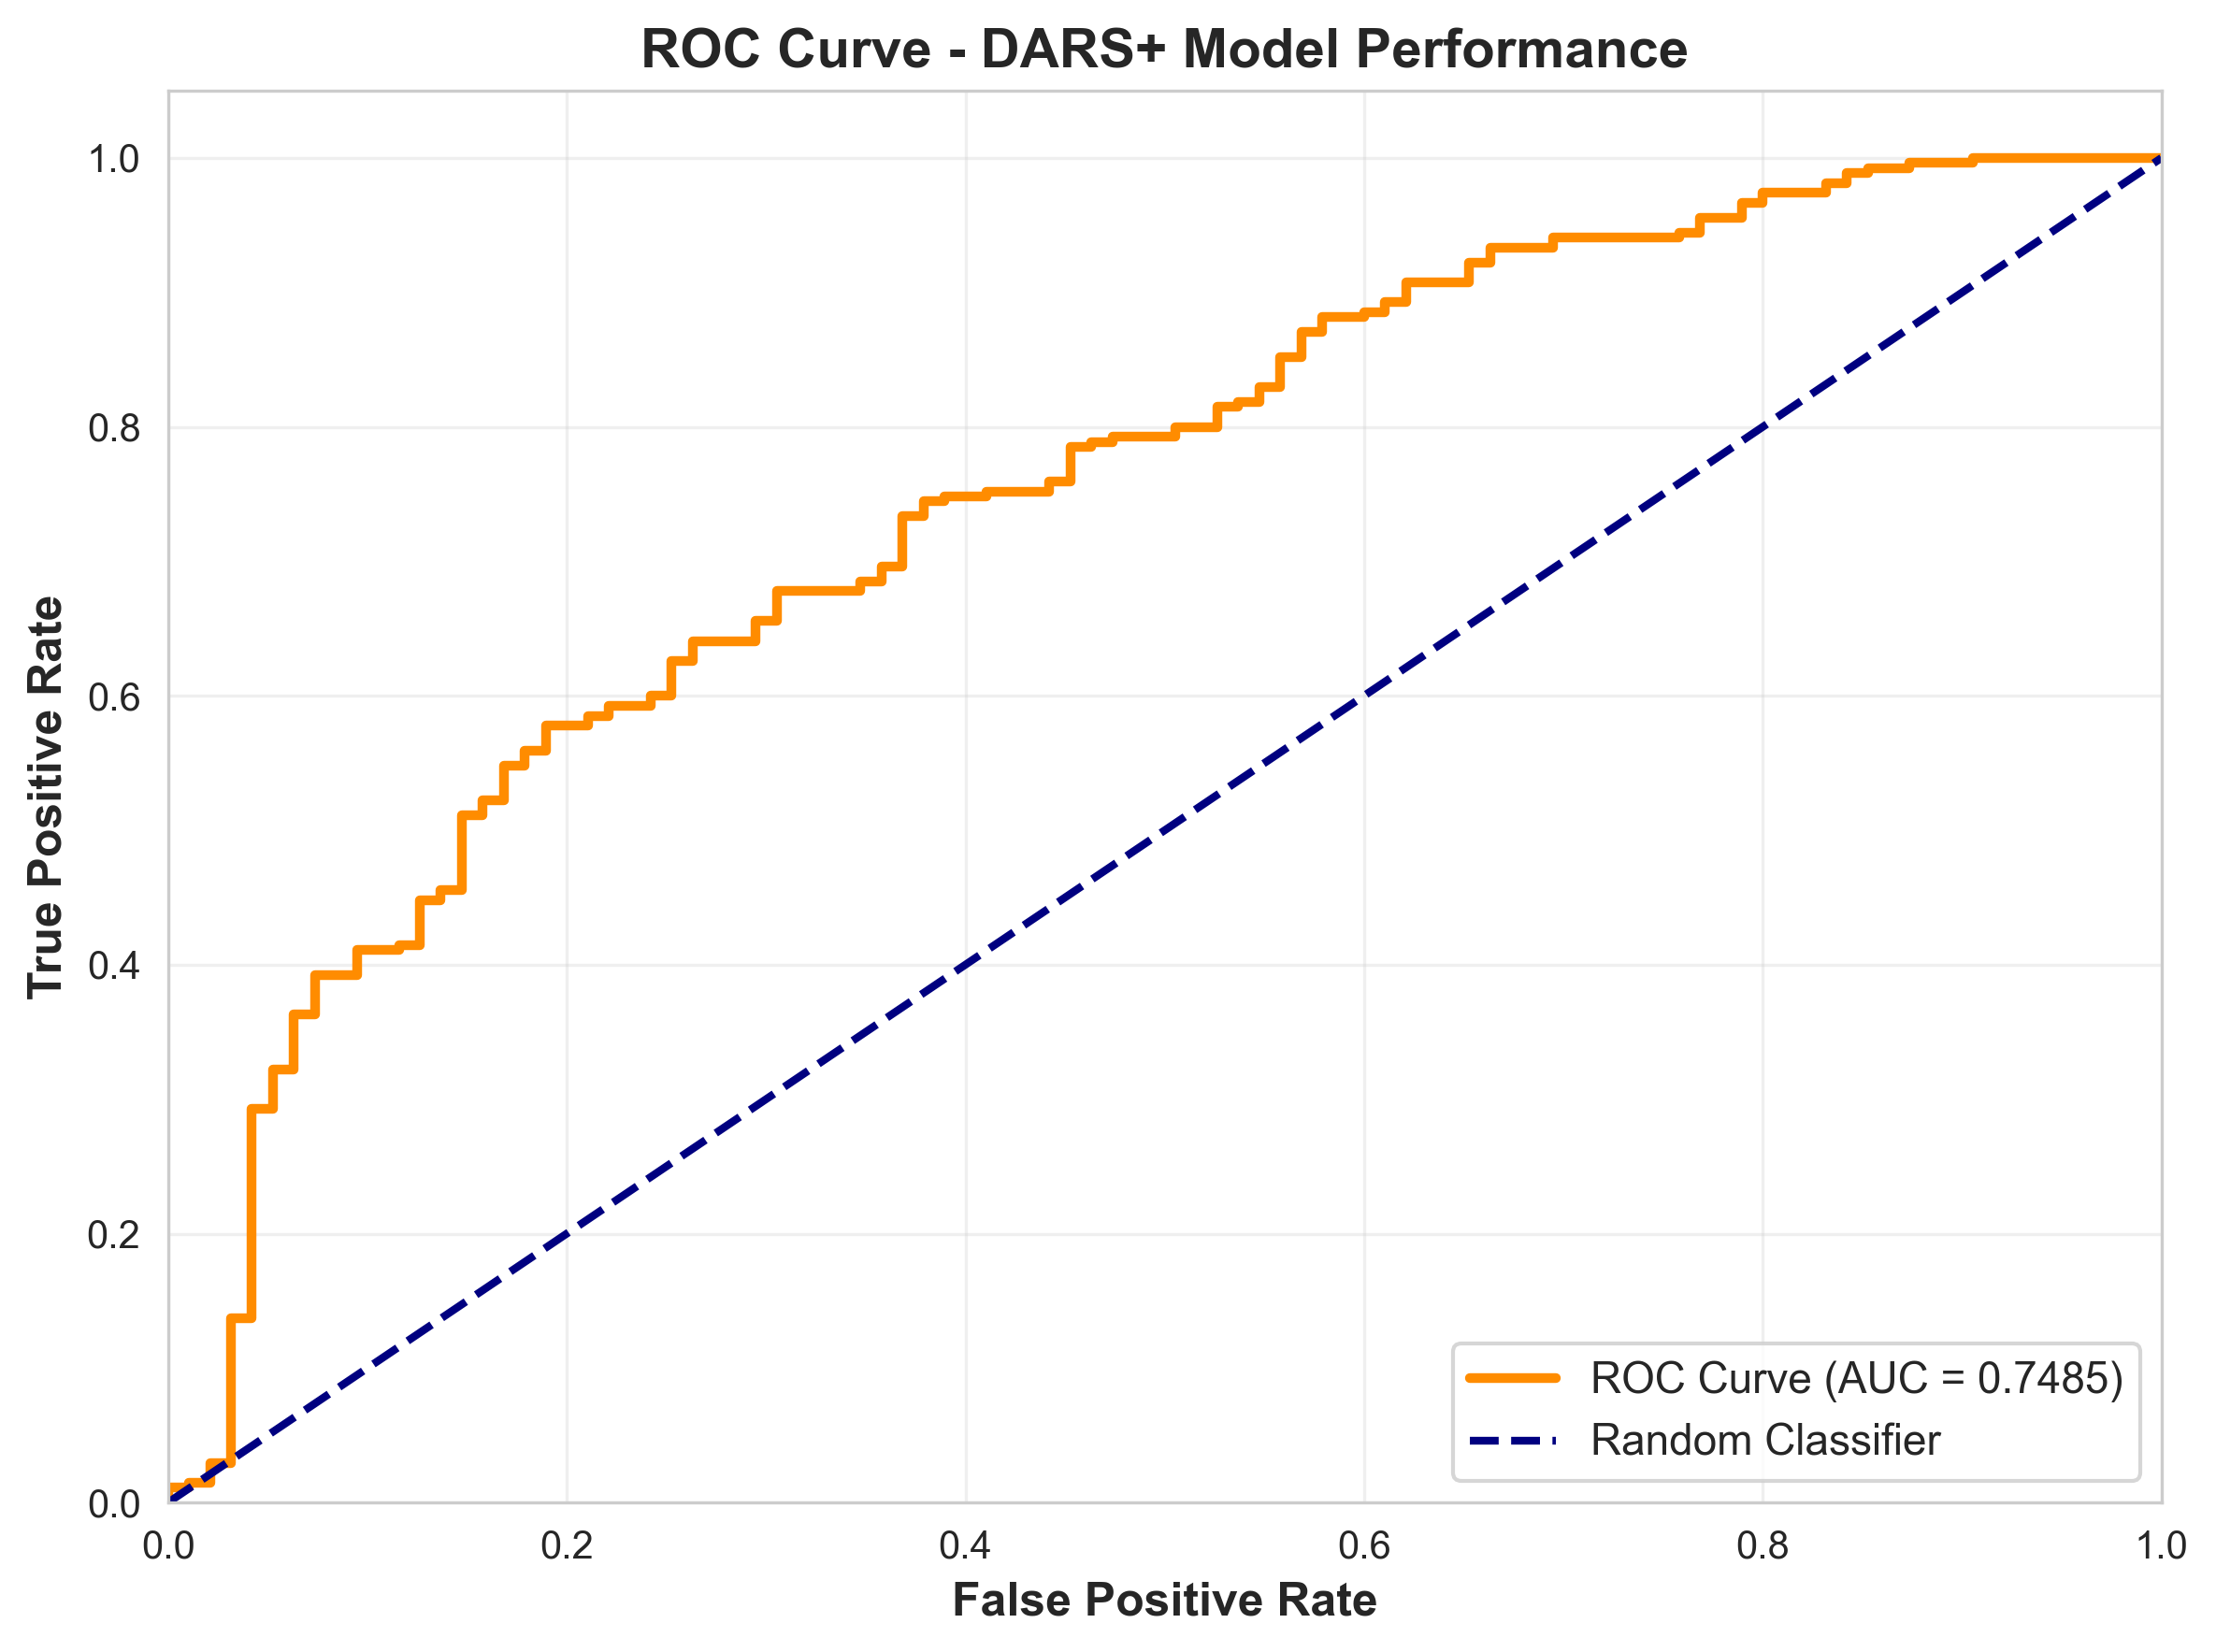
\includegraphics[width=0.45\textwidth]{roc_curve.png}
\caption{ROC curve for DARS difficulty prediction on LeetCode dataset. AUC = 0.7485 demonstrates good separation between easy and hard problems.}
\label{fig:leetcode_roc}
\end{figure}

Dataset analysis revealed that problem frequency (community practice frequency) was the strongest predictor of difficulty ($\beta = +2.29$), followed by difficulty index ($\beta = +0.86$), and surprisingly, engagement factor showed negative association ($\beta = -2.66$), suggesting that highly discussed problems may be well-documented or explained elsewhere. Figure~\ref{fig:leetcode_dashboard} presents a comprehensive performance dashboard including confusion matrix, probability distributions, and feature importance for the LeetCode evaluation. Figure~\ref{fig:leetcode_features} further details the feature importance coefficients.

\begin{figure}[t]
\centering
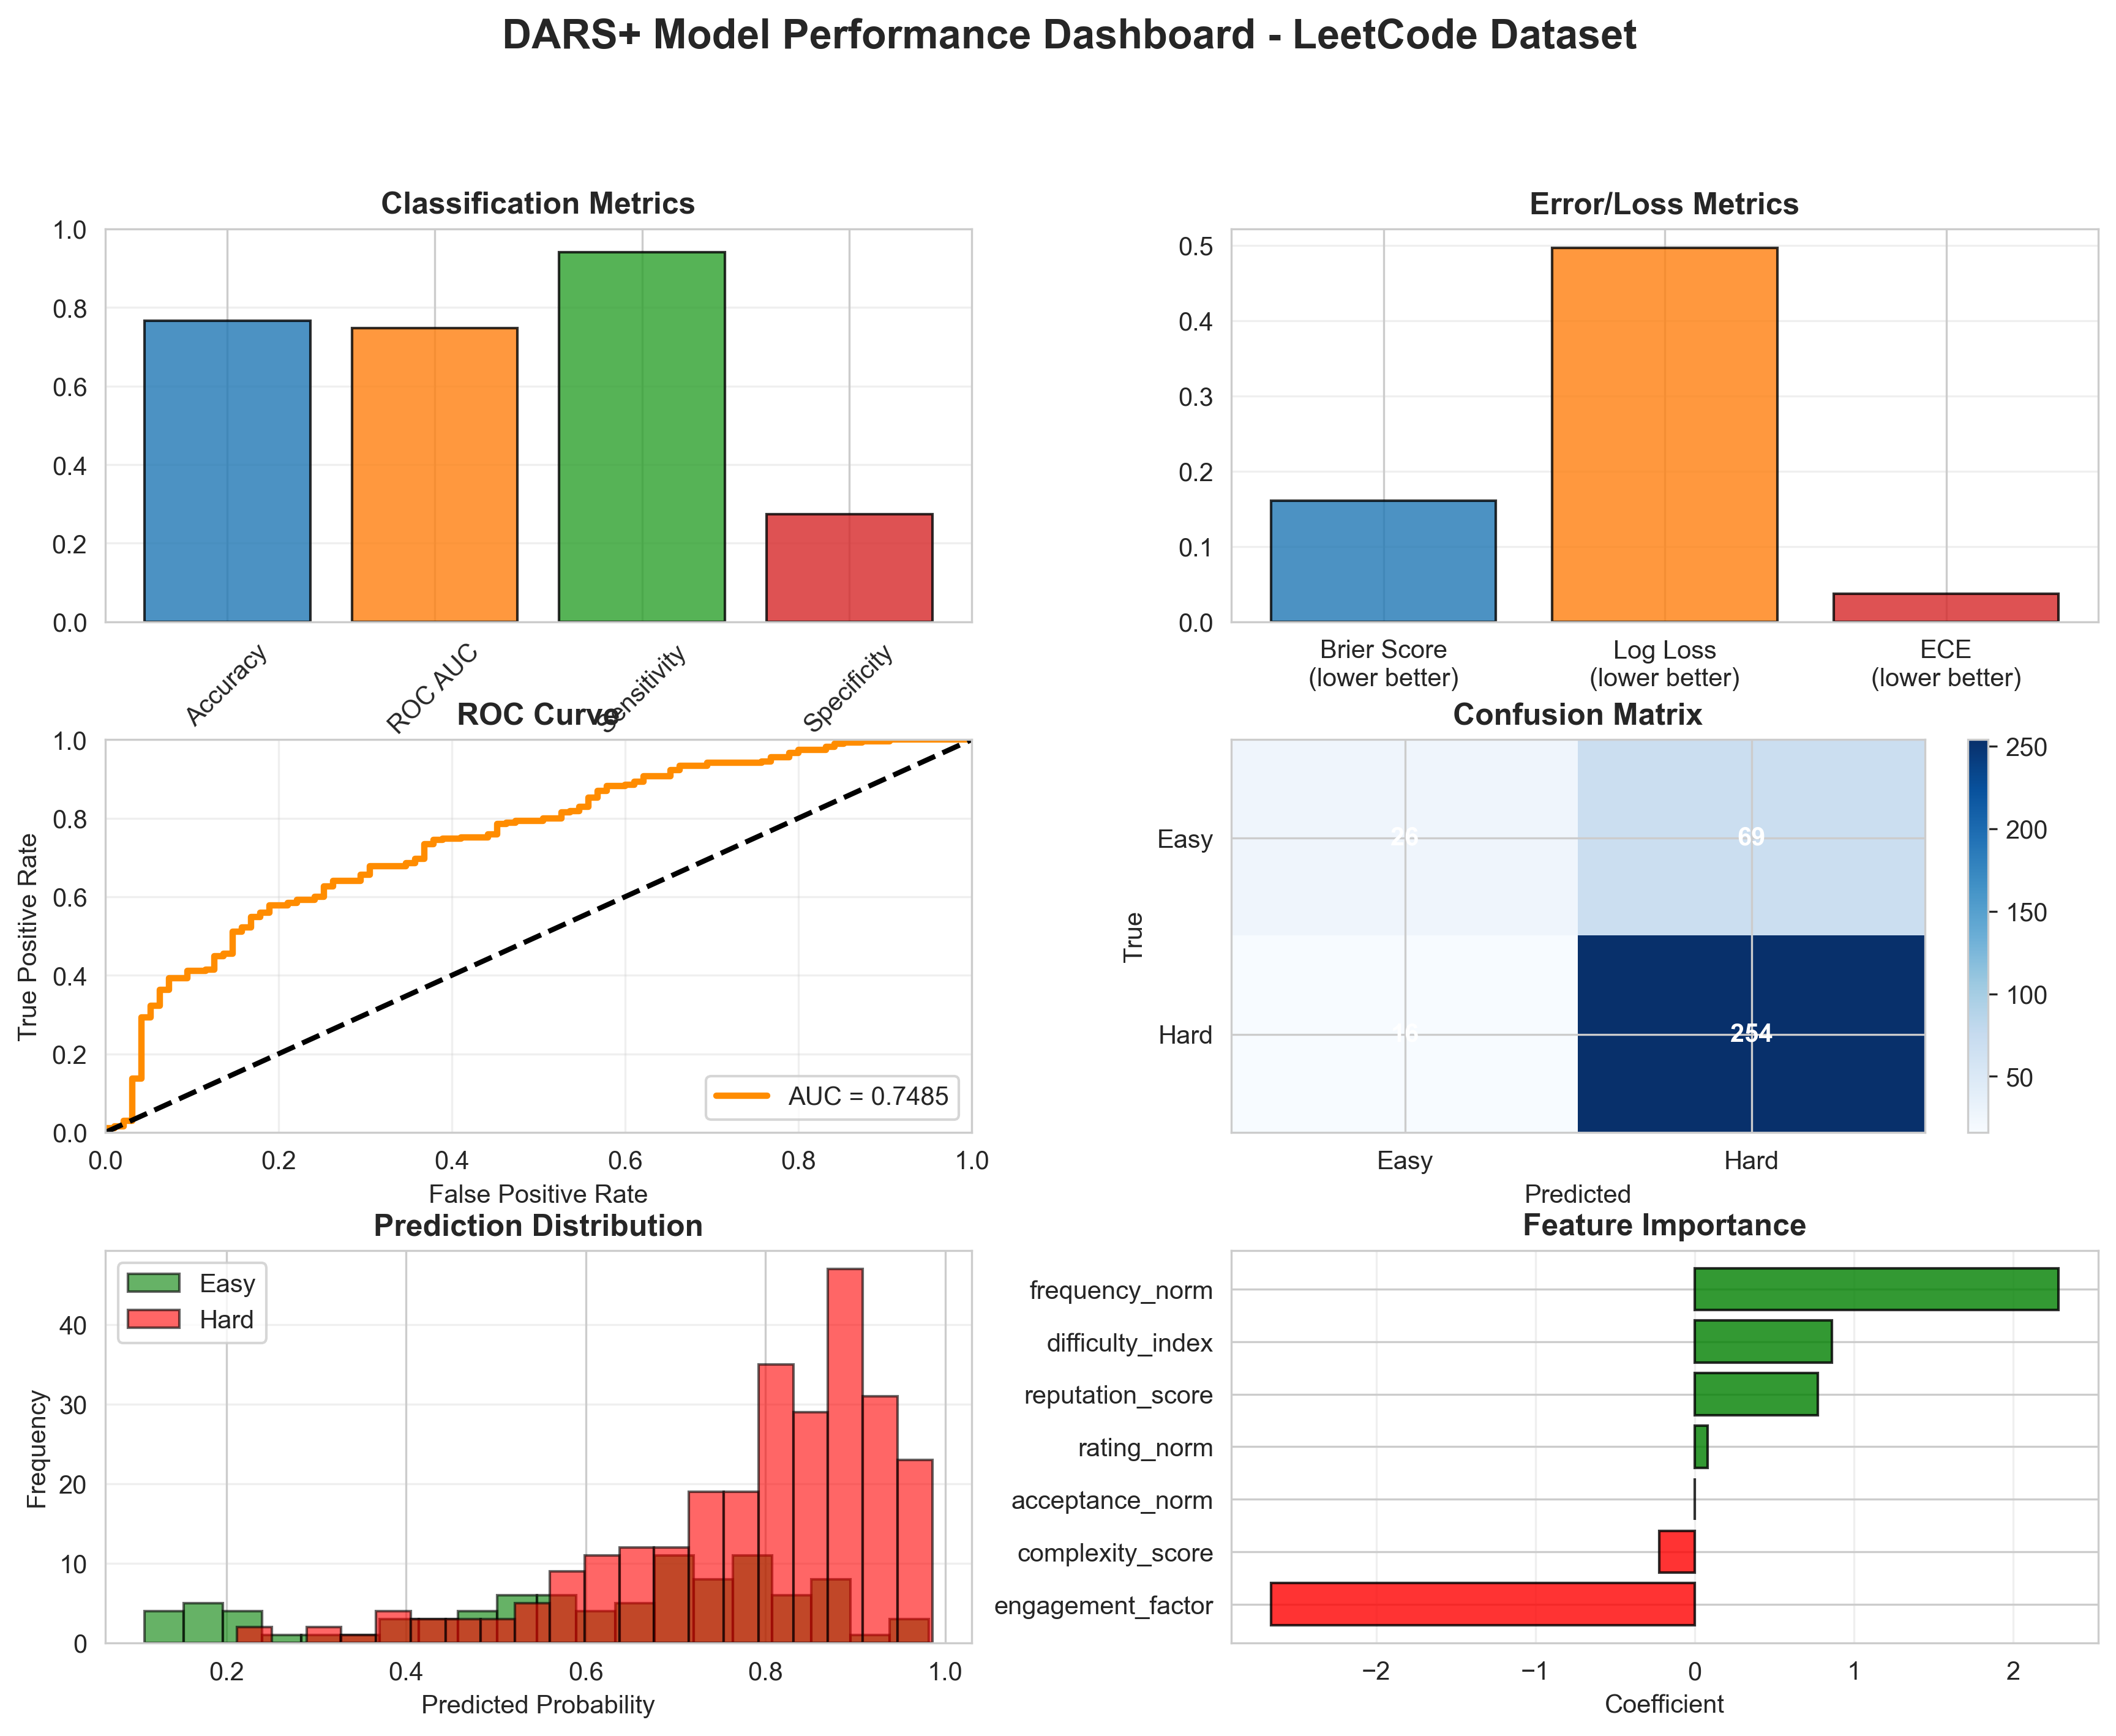
\includegraphics[width=0.45\textwidth]{performance_dashboard.png}
\caption{Comprehensive performance dashboard for DARS on LeetCode dataset showing (1) classification metrics, (2) error metrics, (3) ROC curve, (4) confusion matrix, (5) prediction distribution, and (6) feature importance coefficients.}
\label{fig:leetcode_dashboard}
\end{figure}

\begin{figure}[t]
\centering
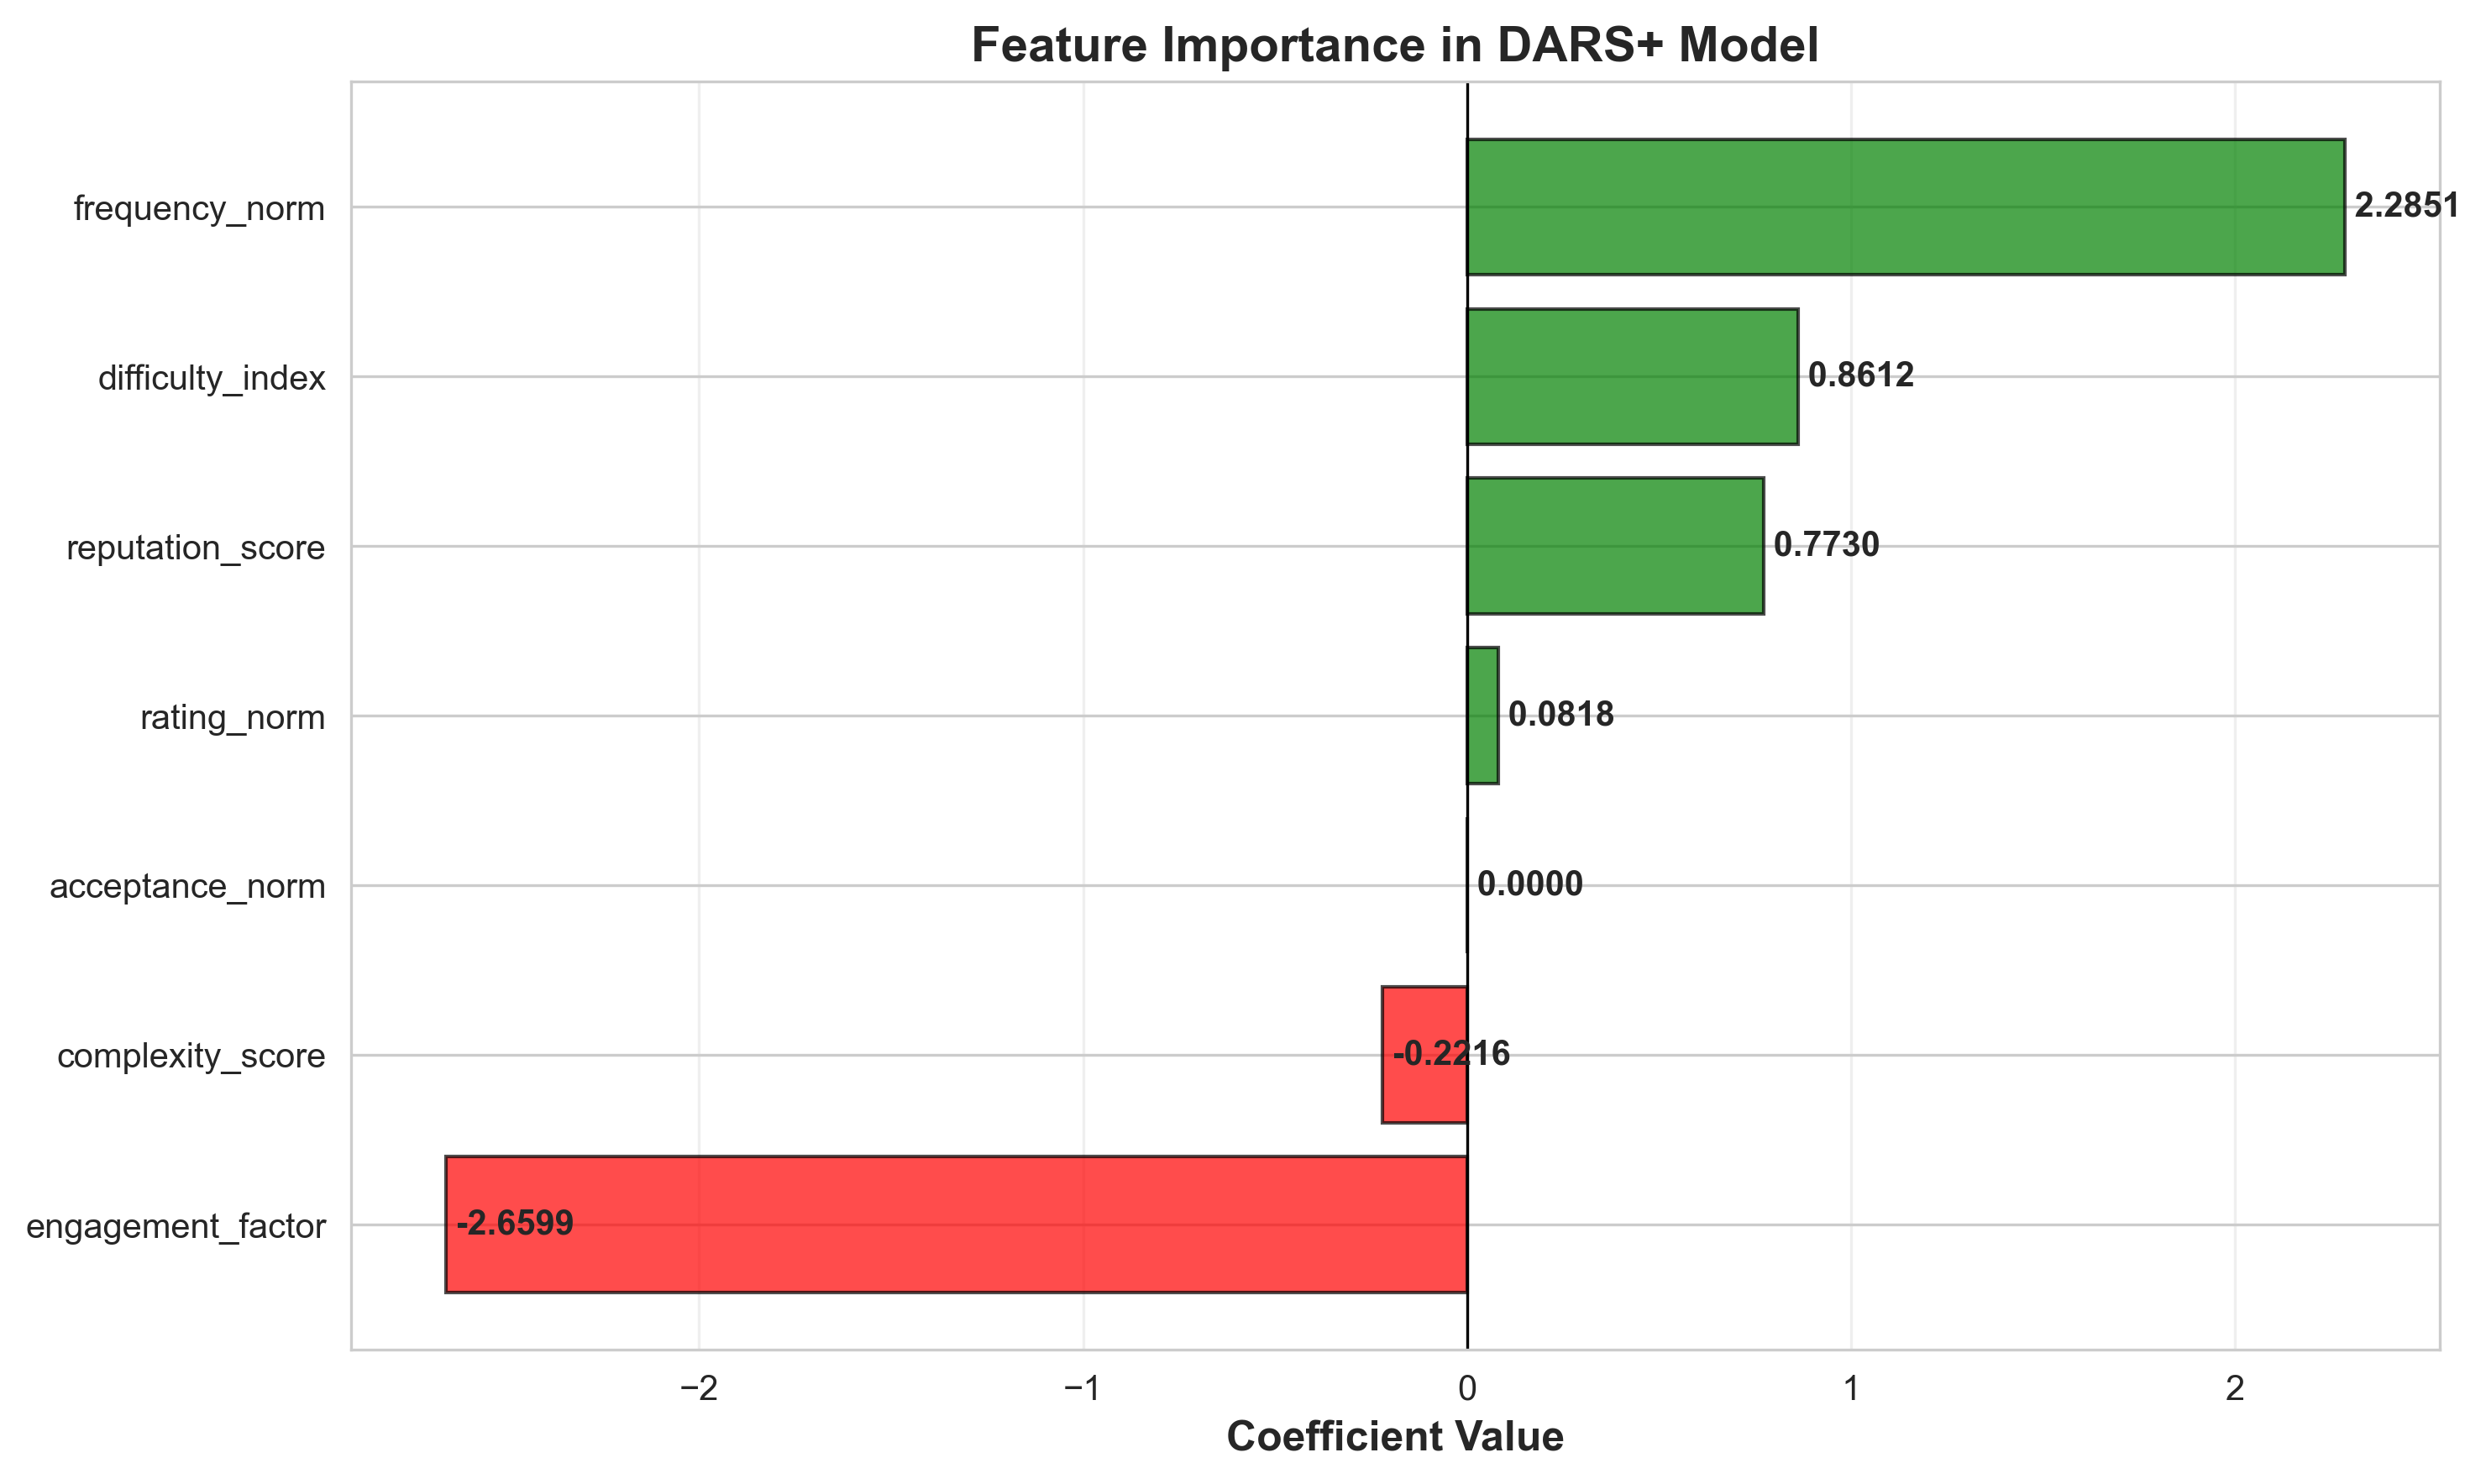
\includegraphics[width=0.45\textwidth]{feature_importance.png}
\caption{Feature importance (logistic regression coefficients) for DARS on LeetCode. Frequency (green, +2.29) is the strongest difficulty predictor, while engagement factor (red, -2.66) negatively predicts difficulty, suggesting well-documented problems are easier for learners.}
\label{fig:leetcode_features}
\end{figure}

\subsection{Additional Knowledge Tracing Baselines}
The current comparison includes only Elo-style and Glicko-2 baselines. Future work should include sequence-model baselines that represent the modern knowledge tracing literature:

\begin{itemize}
    \item \textbf{Bayesian Knowledge Tracing (BKT):} BKT represents learner mastery as a hidden Markov model with hidden and observed states. It explicitly models the probability of learning, forgetting, guessing, and slipping. BKT is well-established and has a long history in educational data mining. However, BKT typically assumes a fixed set of skills and does not naturally incorporate item-specific difficulty or graph structure.
    
    \item \textbf{Deep Knowledge Tracing (DKT):} DKT uses recurrent neural networks (LSTM) to encode sequences of (problem, correctness) pairs and predict the next outcome. DKT is powerful but produces latent states that are difficult to interpret. It also typically ignores response-process information such as hints, response time, and attempts unless explicitly added to the input embedding.
    
    \item \textbf{Self-Attentive Knowledge Tracing (SAKT):} SAKT improves on DKT by using multi-head self-attention to identify relevant past interactions. This allows the model to weight distant interactions more heavily if they are conceptually similar to the current attempt. SAKT often outperforms DKT but remains opaque and requires careful feature engineering for hints and time.
    
    \item \textbf{Graph Neural Knowledge Tracing (GNKT):} GNKT embeds problems and skills as nodes in a graph and uses graph convolutions to propagate information. This is conceptually aligned with DARS's graph-guided approach, but GNKT typically uses learned embeddings rather than interpretable rating scales. Comparing GNKT against DARS would test whether learned graph representations or explicit skill graphs better serve adaptive assessment.
\end{itemize}

All baselines should be evaluated under the same chronological online-replay protocol to ensure fair comparison.

\subsection{Graph Construction Strategies}
The current DARS evaluation uses item-skill tags and temporal co-occurrence to infer edges. Future work should systematically compare multiple graph construction strategies:

\begin{itemize}
    \item \textbf{Skill-Only Graph:} Nodes are skills; edges connect skills that frequently co-occur in problems or that form prerequisite-like relationships. This is the most interpretable but may miss item-specific information.
    
    \item \textbf{Temporal Transition Graph:} Nodes are problems; edges are weighted by how often one problem is followed by another in actual learner sequences. This graph directly reflects pedagogical flow but may be noisy or brittle if the underlying routing policy has biases.
    
    \item \textbf{Expert Prerequisite Graph:} Nodes are problems or skills; edges are manually authored by curriculum experts to encode known prerequisites. This is expensive but highly reliable. It also makes remediation recommendations easier to justify.
    
    \item \textbf{Hybrid Graph:} A weighted combination of skill, temporal, and expert information. The weights can be tuned to maximize prediction quality or learning outcomes on a validation set.
\end{itemize}

Each graph strategy should be evaluated on the same ASSISTments and LeetCode datasets to measure the impact of graph quality on routing and prediction performance.

\subsection{Fairness and Robustness Analysis}
Assessment systems must be fair and robust. Future work should analyze DARS performance across several dimensions:

\begin{itemize}
    \item \textbf{Learner Group Fairness:} Evaluate whether DARS shows consistent calibration and ranking quality across learner demographics (e.g., grade level, subject, geographic region if available). Fairness metrics should include equal opportunity (equal true positive rates across groups), demographic parity, and calibration parity.
    
    \item \textbf{Skill Category Analysis:} Some skill categories may be harder to predict than others (e.g., procedural skills vs.\ conceptual skills). DARS should be evaluated separately by skill type to ensure that the algorithm does not systematically underestimate or overestimate ability in certain domains.
    
    \item \textbf{Cold-Start Robustness:} Learners with few prior attempts are especially vulnerable to noisy early estimates. DARS's dynamic $K$-factor is designed to handle this, but explicit evaluation on cold-start learners (those with $<5$ or $<10$ total attempts) should measure how quickly the system converges to accurate estimates and whether rating oscillations or remediation loops harm learning.
    
    \item \textbf{Adversarial and Distribution Shift:} What happens if learner behavior changes (e.g., guess-and-check vs.\ deliberate practice)? Does DARS recover or does it lock in misestimates? How does DARS perform on out-of-distribution problems or skills not seen during calibration?
\end{itemize}

Figure~\ref{fig:leetcode_calibration} shows calibration across confidence bins for LeetCode; similar stratified calibration analysis should be extended to fairness-sensitive learner and skill groups.

\begin{figure}[t]
\centering
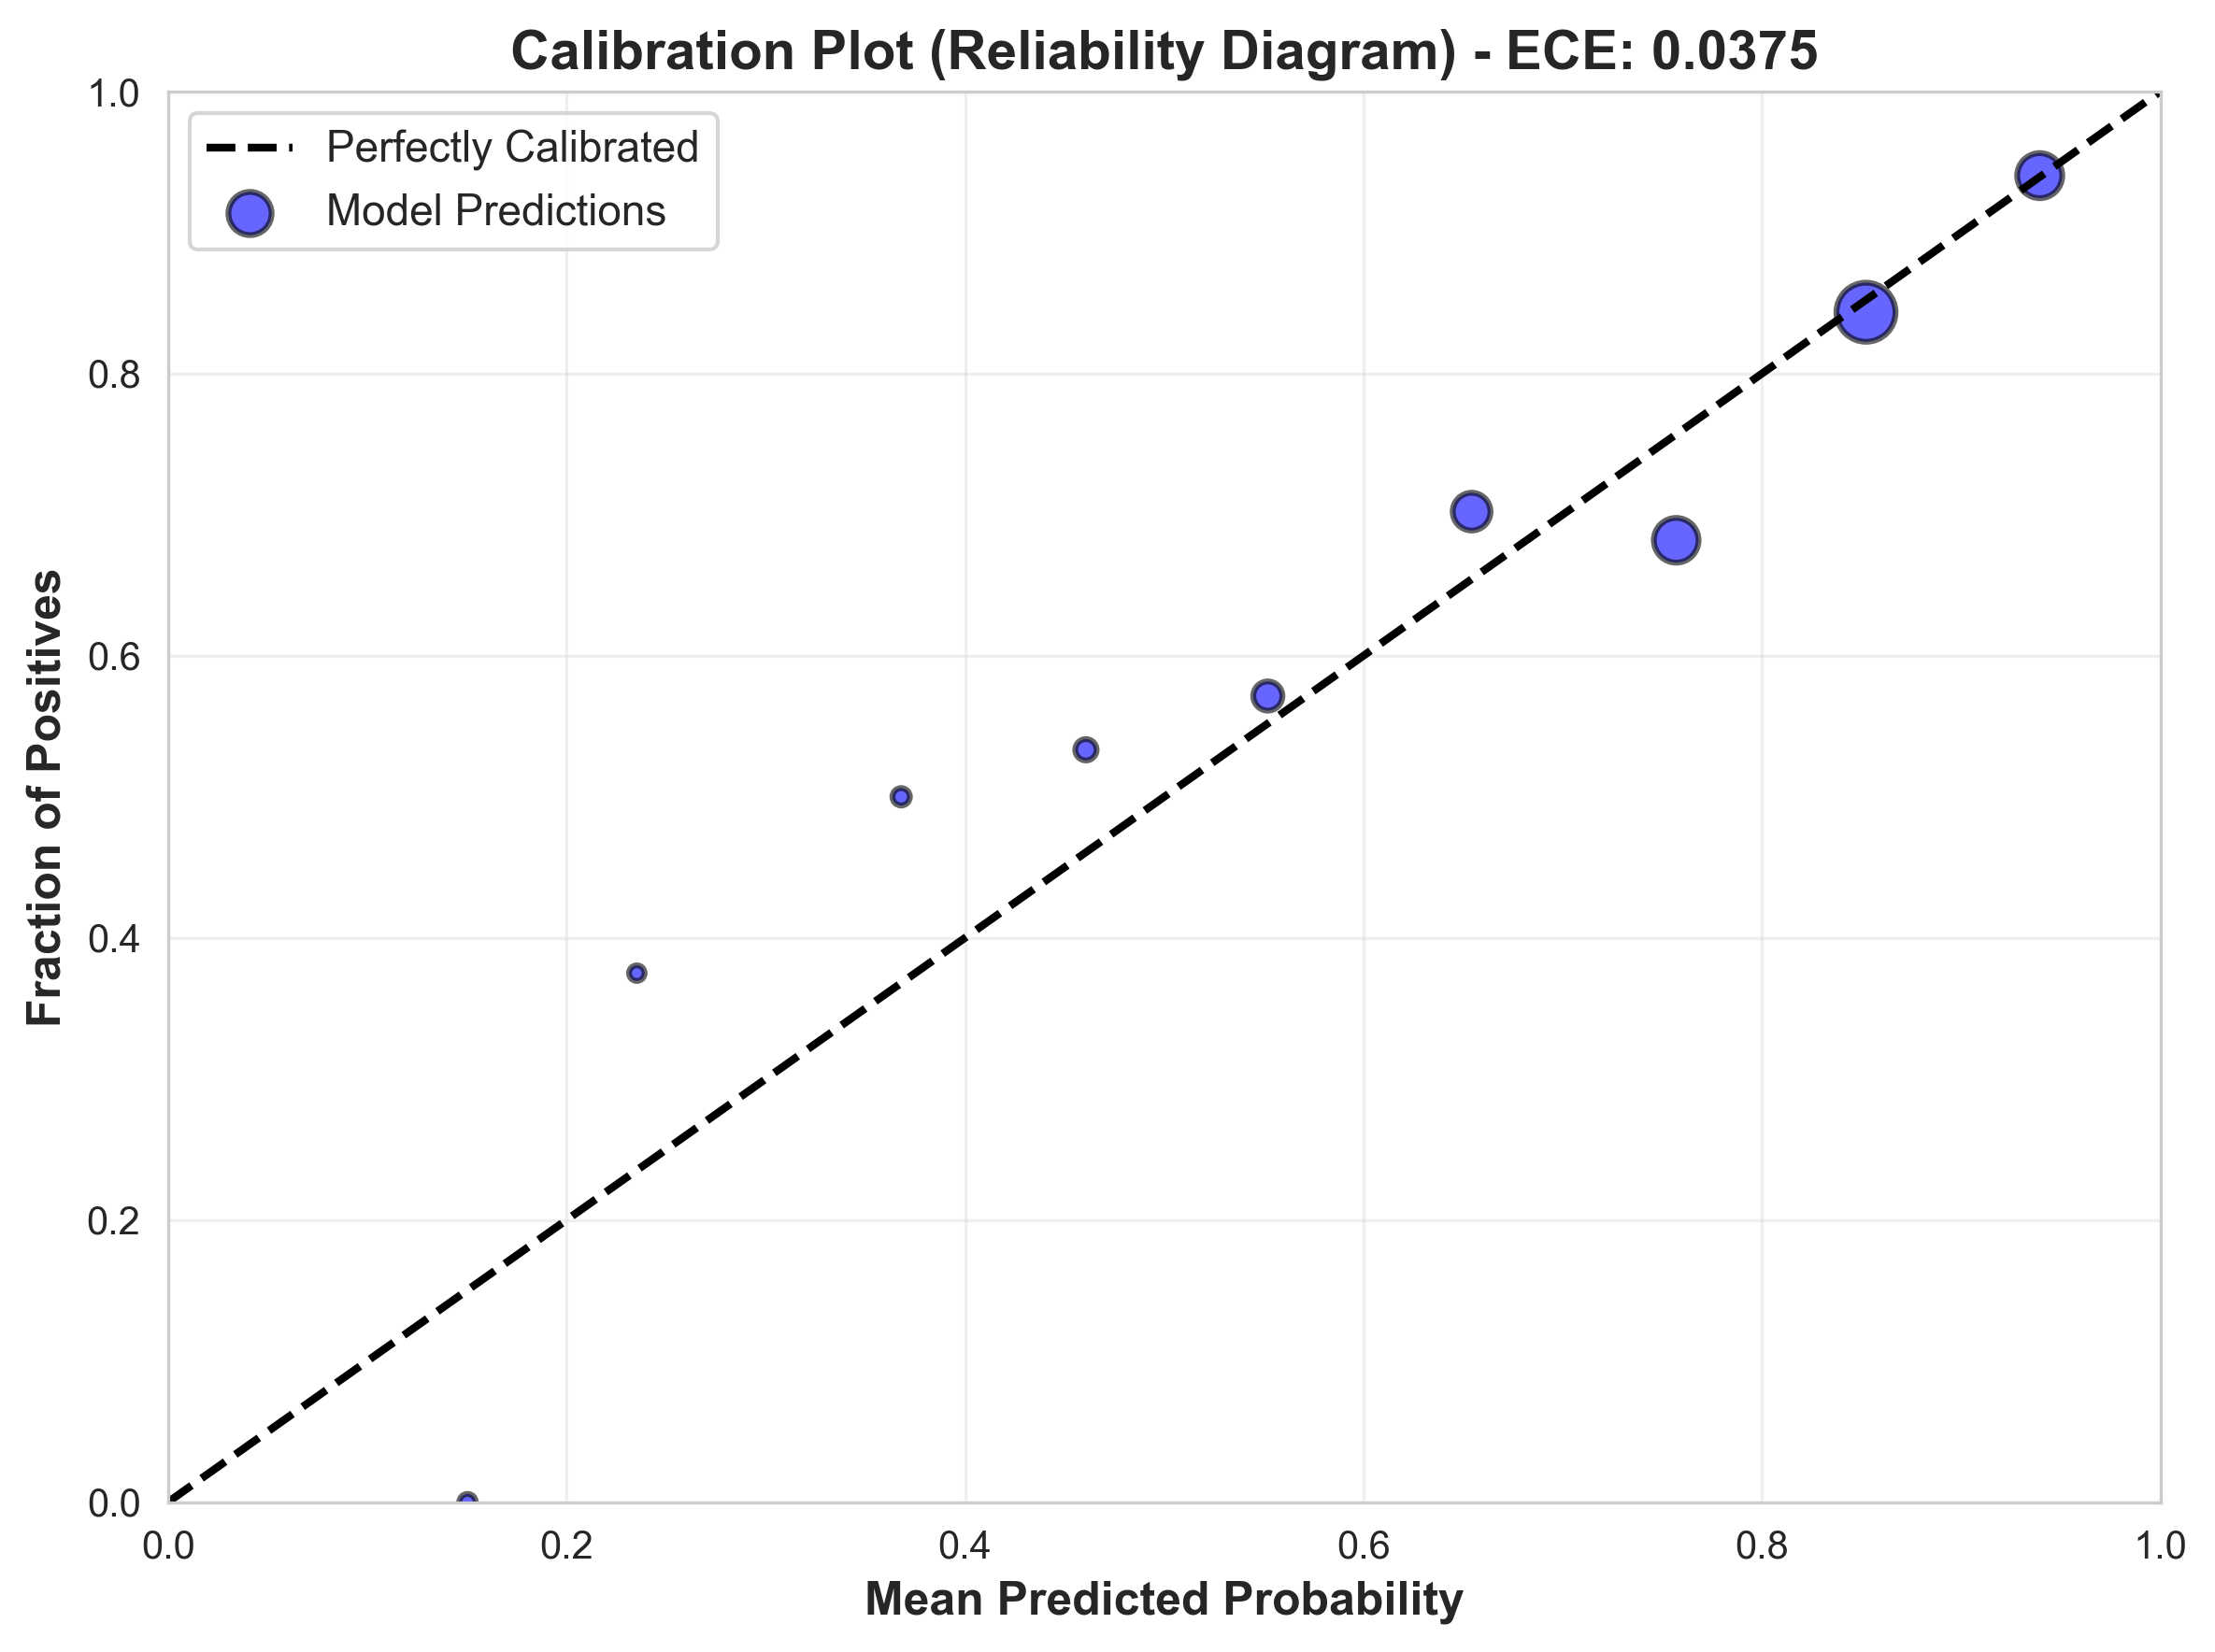
\includegraphics[width=0.45\textwidth]{calibration_plot.png}
\caption{Calibration plot (reliability diagram) for LeetCode dataset. Points lie near the diagonal, indicating good agreement between predicted probability and observed frequency. ECE = 0.0375.}
\label{fig:leetcode_calibration}
\end{figure}

\subsection{Cross-Dataset Validation}
The current evaluation uses only ASSISTments. LeetCode offers a contrasting domain: algorithm problems with clear acceptance rates rather than tutoring-system hints. Future work should train and evaluate DARS on multiple independent educational datasets (e.g., ASSISTments, LeetCode, Coursera, edX, Khan Academy if available) to test generalization of learned calibration parameters and graph strategies across platforms and learner populations. Figures~\ref{fig:leetcode_confusion} and~\ref{fig:leetcode_metrics} summarize LeetCode evaluation results.

\begin{figure}[t]
\centering
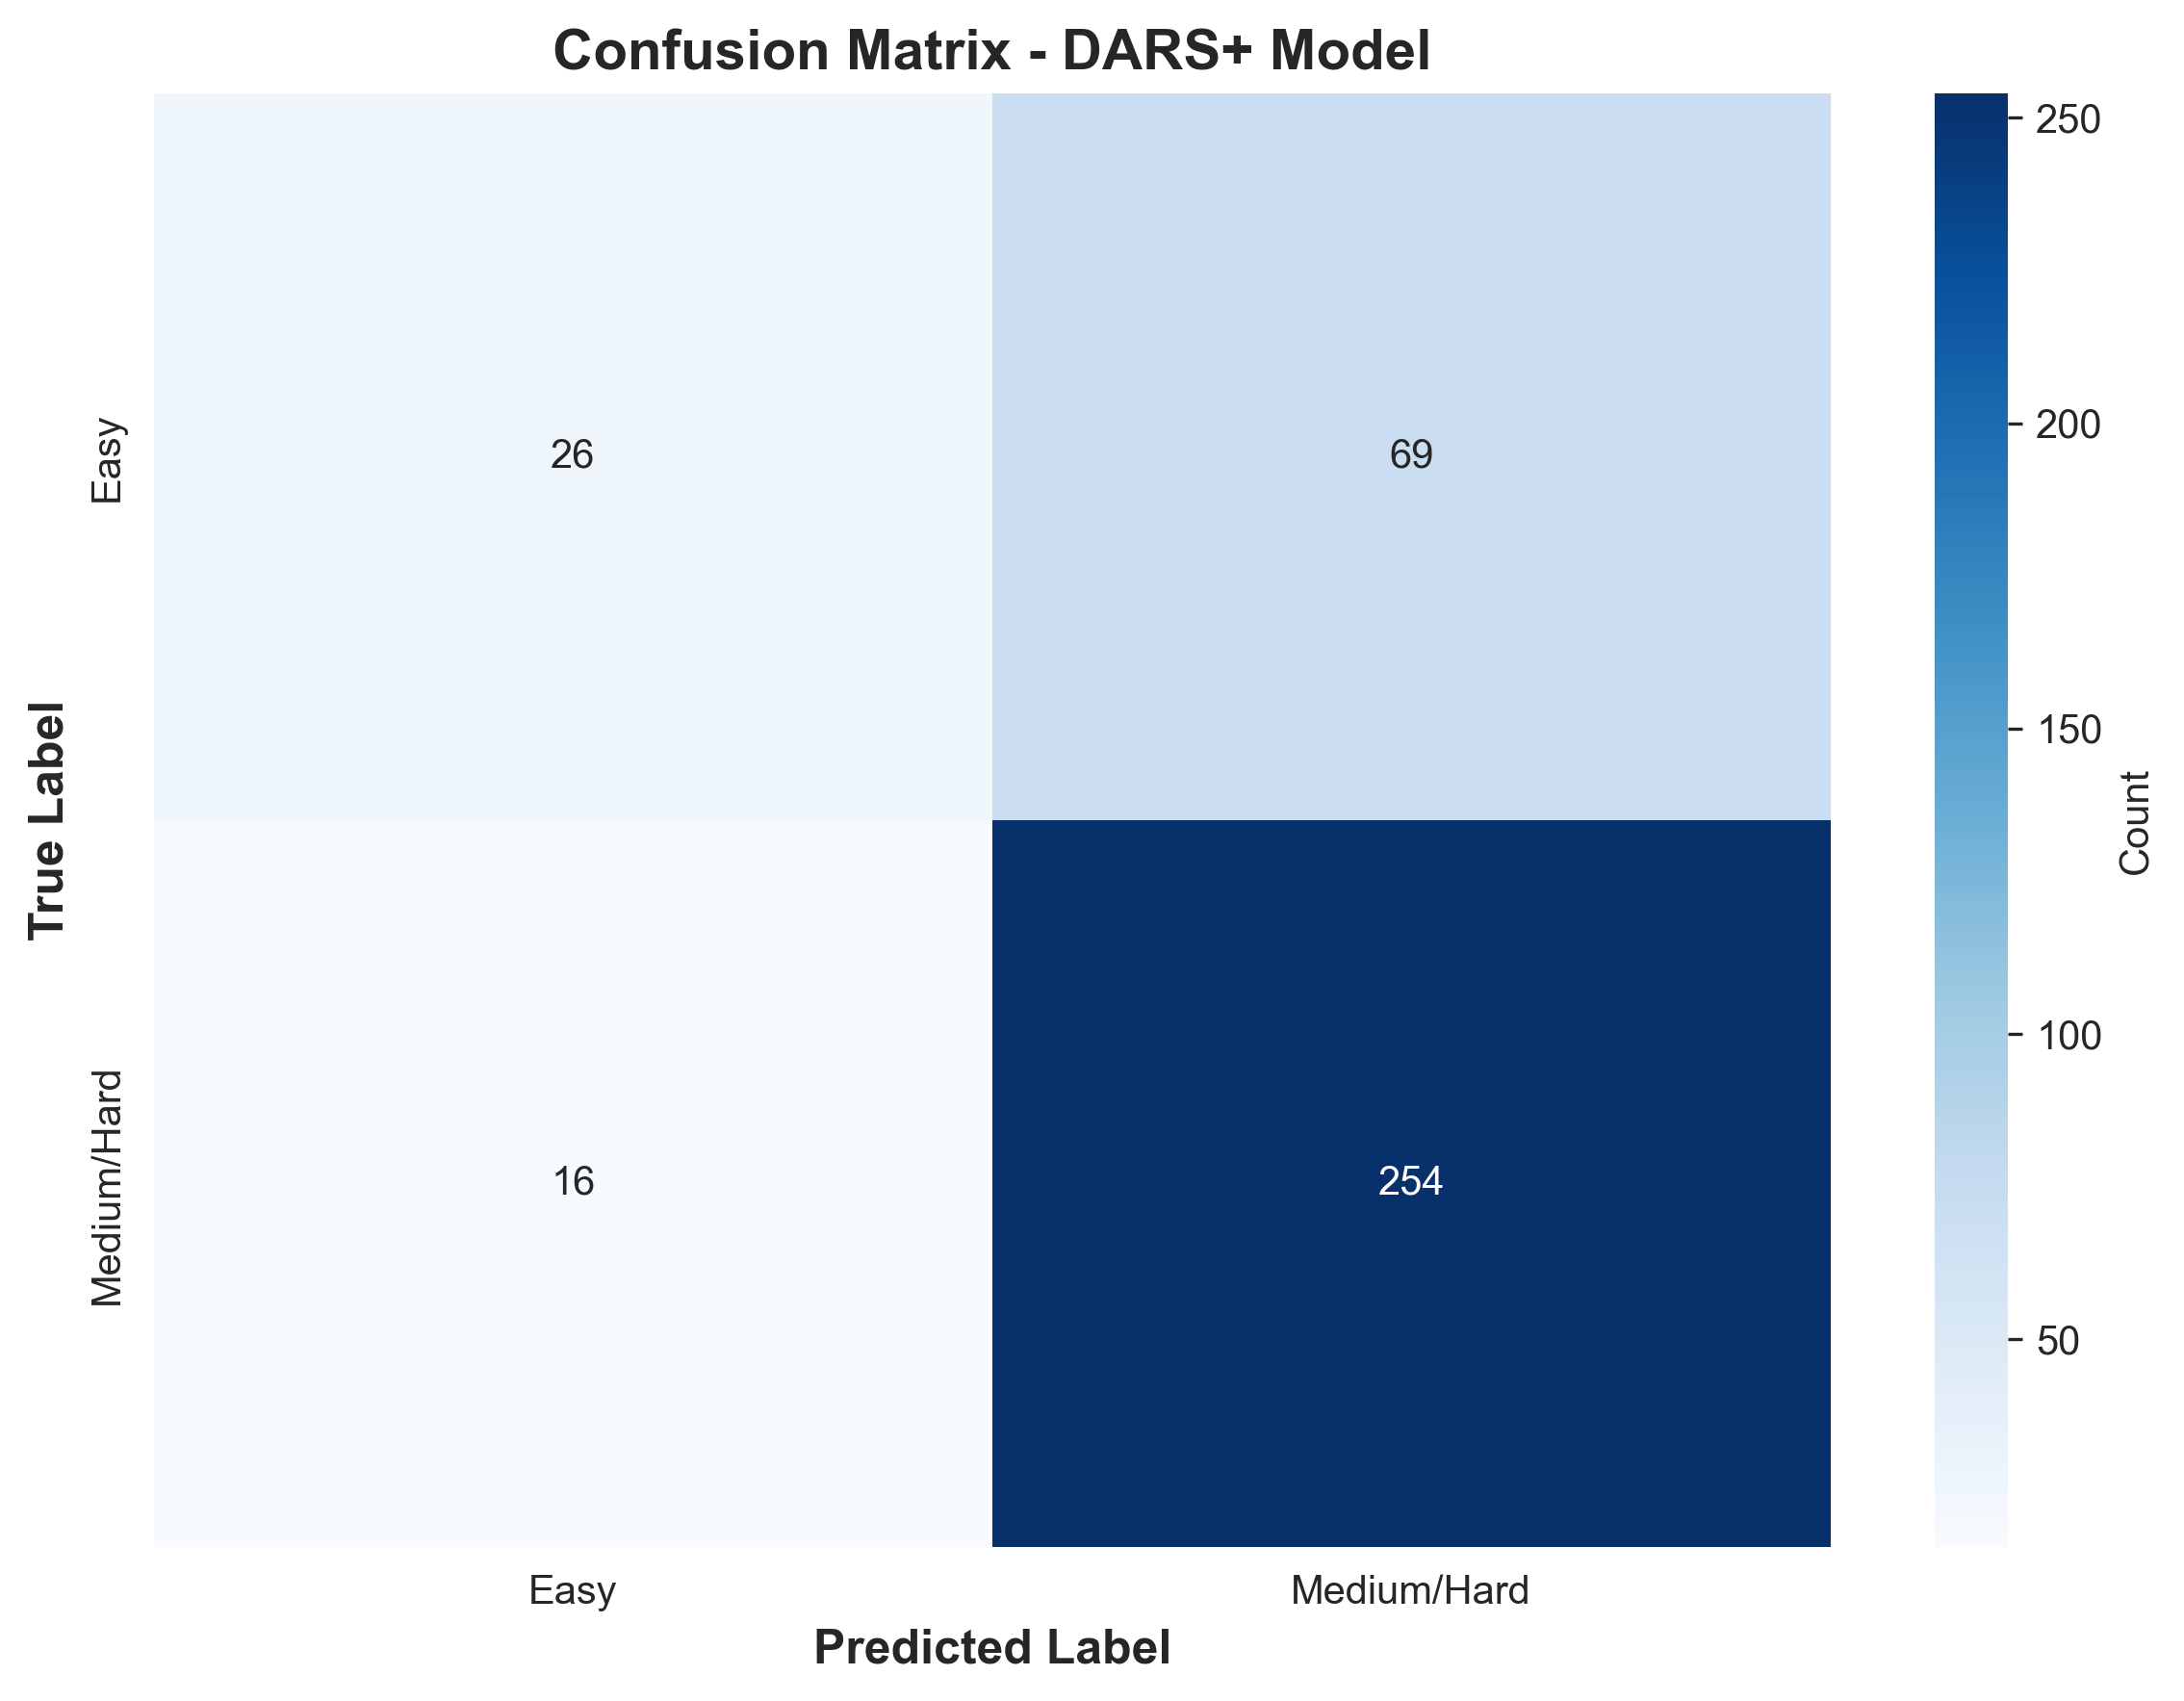
\includegraphics[width=0.45\textwidth]{confusion_matrix.png}
\caption{Confusion matrix for DARS on LeetCode. The model achieved high sensitivity (94.07\% true positive rate for hard problems) but lower specificity (27.37\%), indicating a bias toward predicting problems as hard.}
\label{fig:leetcode_confusion}
\end{figure}

\begin{figure}[t]
\centering
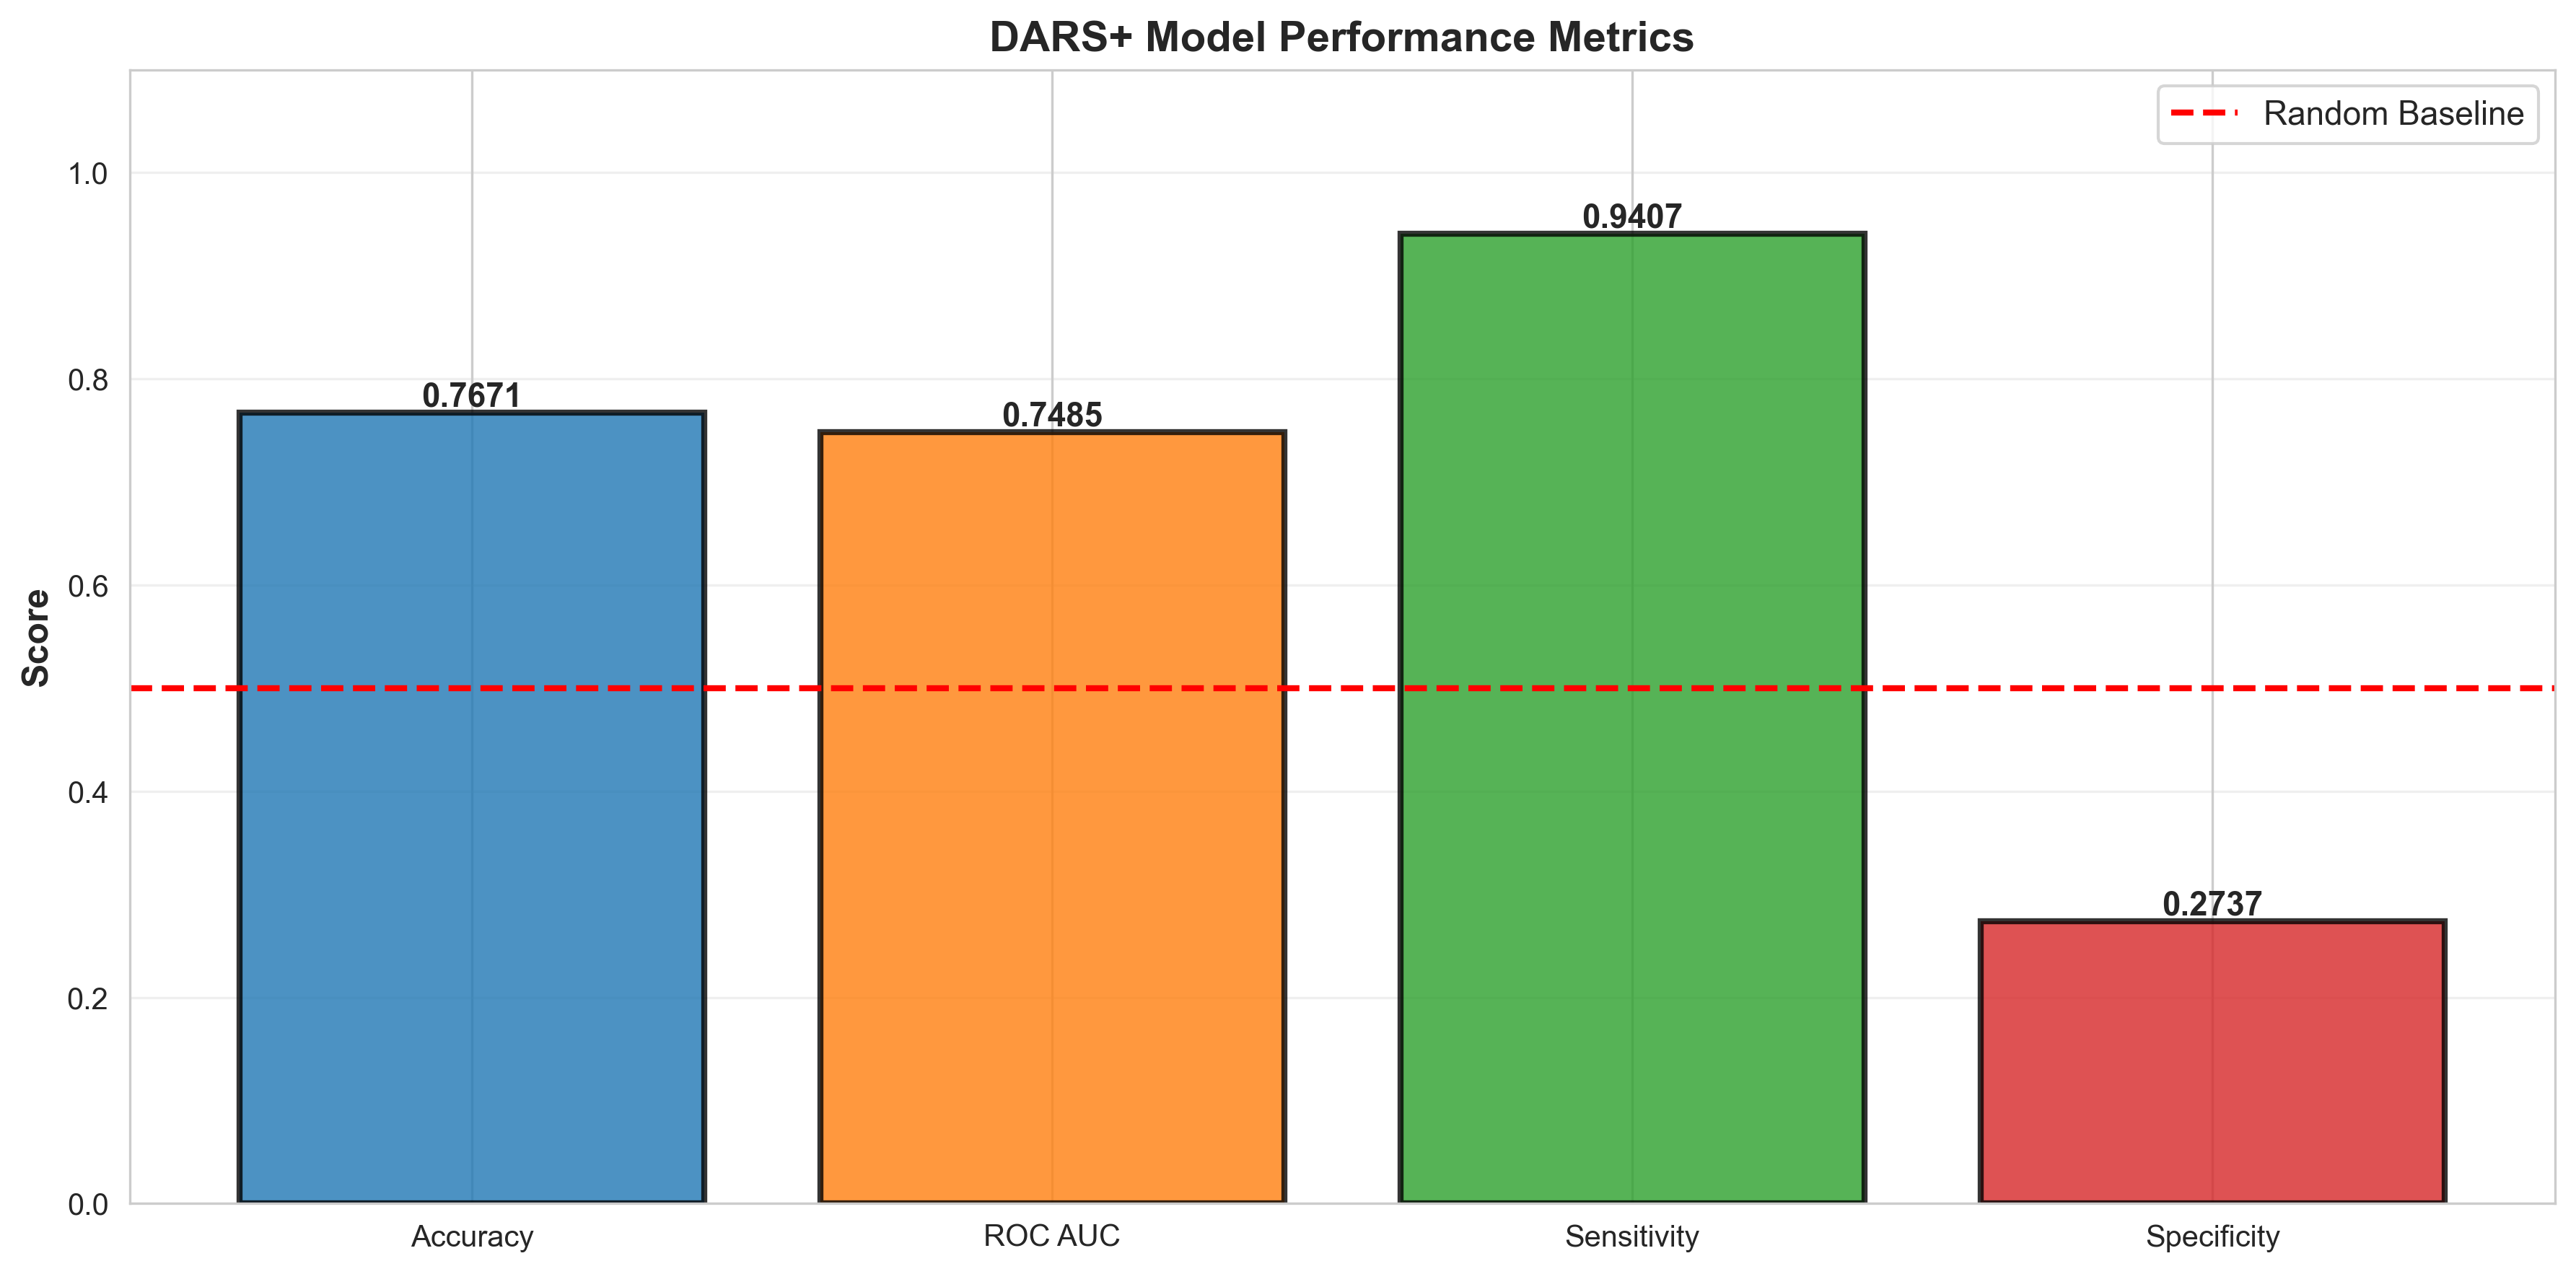
\includegraphics[width=0.45\textwidth]{metrics_comparison.png}
\caption{Performance metrics comparison on LeetCode dataset. Accuracy, ROC AUC, sensitivity, and specificity demonstrate strong overall ranking and classification ability.}
\label{fig:leetcode_metrics}
\end{figure}

\begin{figure}[t]
\centering
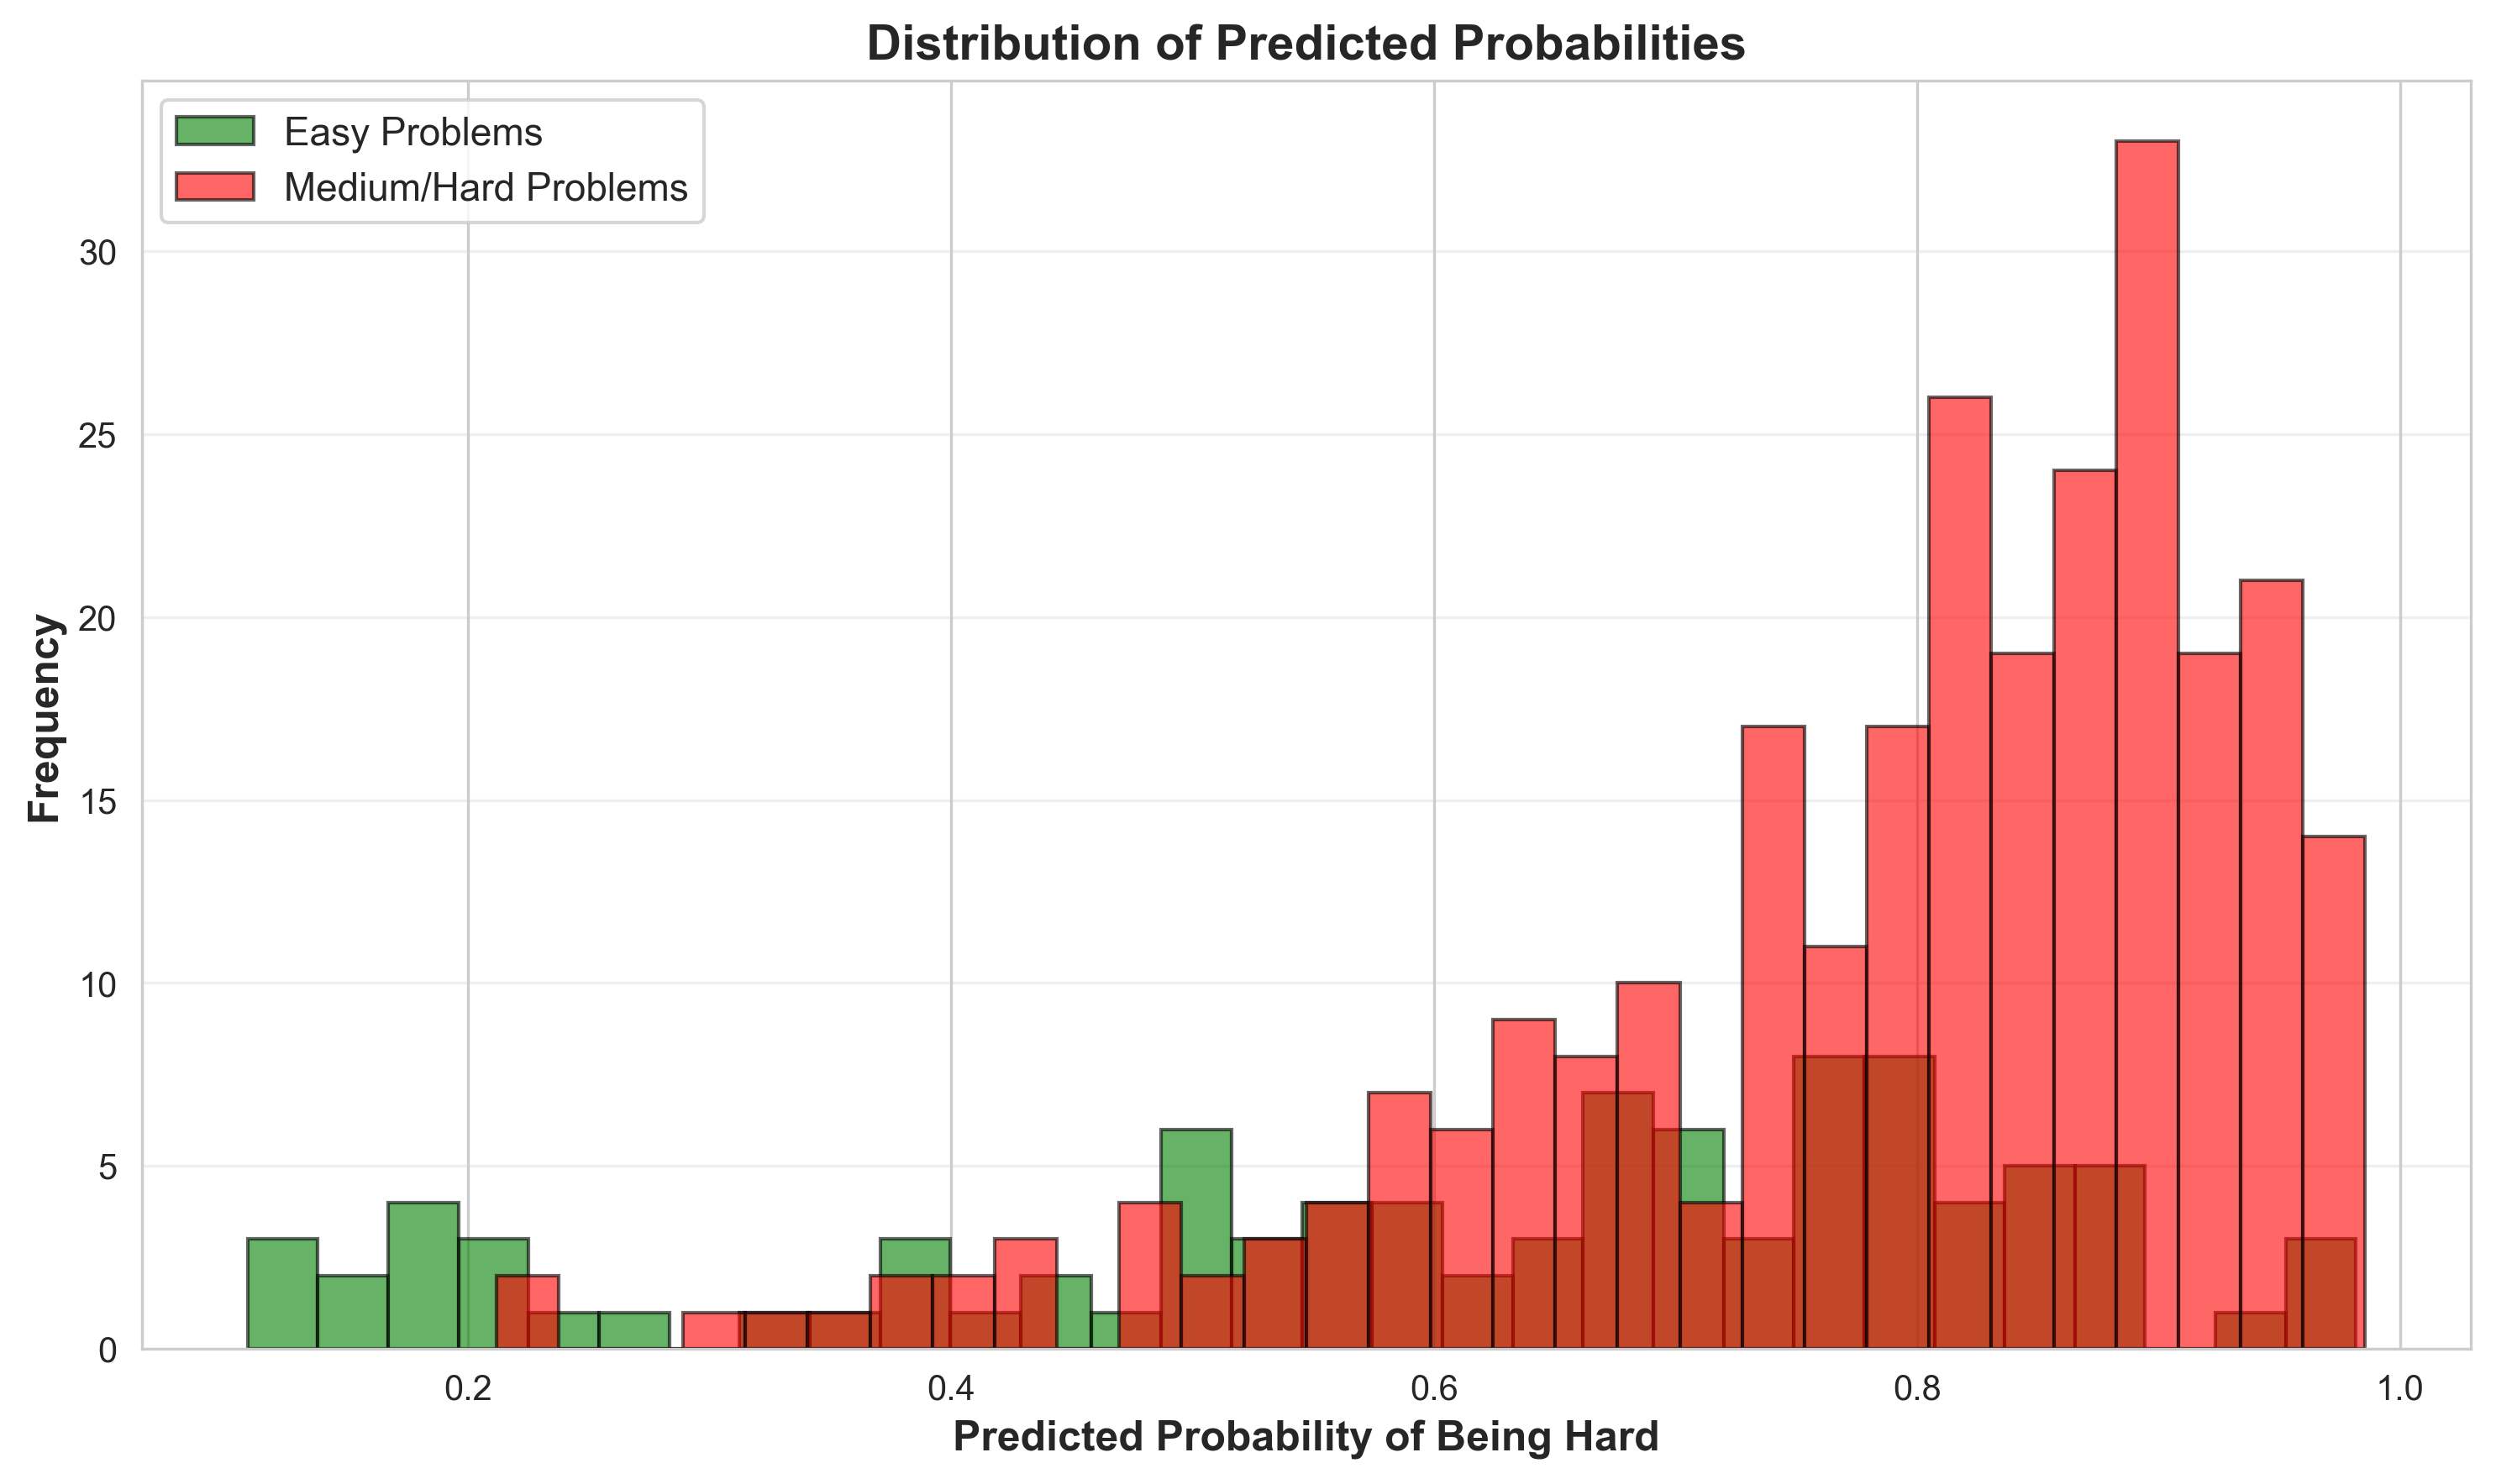
\includegraphics[width=0.45\textwidth]{probability_distribution.png}
\caption{Prediction probability distribution on LeetCode dataset. Green histogram shows predicted probabilities for easy problems; red histogram shows predicted probabilities for hard problems. Clear separation indicates good model discrimination.}
\label{fig:leetcode_probdist}
\end{figure}

\section{Conclusion}
This paper presented DARS, a Dynamic Adaptive Rating System for graph-guided assessment and remediation. DARS extends online rating with response-quality scoring, dynamic update control, graph-aware item difficulty, remediation routing, and calibrated probability estimation. On the ASSISTments 2012-2013 dataset, DARS outperforms static mastery, fixed-$K$ Elo, and Glicko-2 on Brier score, log loss, accuracy, and ROC AUC while maintaining low calibration error.

Additionally, preliminary evaluation on the LeetCode dataset demonstrates DARS applicability to problem difficulty prediction in coding-assessment domains, achieving 76.71\% accuracy and 0.7485 ROC AUC with well-calibrated predictions (ECE = 0.0375). The LeetCode results suggest that DARS principles of feature-driven difficulty modeling and response-aware calibration extend beyond tutoring systems to open online coding platforms.

The result is an interpretable and deployable algorithmic framework for industry assessment systems that require both accurate scoring and actionable personalization across diverse educational domains. Future work should include live learning-outcome studies, additional knowledge-tracing baselines, systematic graph construction strategies, and fairness analysis across learner populations.

\section*{Acknowledgment}
The author thanks the maintainers of the ASSISTments ecosystem for making large-scale educational interaction data available for research.

\begin{thebibliography}{00}
\bibitem{elo}
A. E. Elo, \textit{The Rating of Chessplayers, Past and Present}. New York, NY, USA: Arco, 1978.

\bibitem{glickman2008glicko2}
M. E. Glickman, ``Rating systems for all sports,'' \textit{Journal of Quantitative Analysis in Sports}, vol. 4, no. 3, 2008.

\bibitem{corbett1994bkt}
A. T. Corbett and J. R. Anderson, ``Knowledge tracing: Modeling the acquisition of procedural knowledge,'' \textit{User Modeling and User-Adapted Interaction}, vol. 4, no. 4, pp. 253--278, 1994.

\bibitem{piech2015dkt}
C. Piech, J. Spencer, J. Huang, S. Ganguli, M. Sahami, L. Guibas, and J. Sohl-Dickstein, ``Deep knowledge tracing,'' in \textit{Proc. 28th Conf. Neural Information Processing Systems}, 2015, pp. 505--513.

\bibitem{pandey2019sakt}
S. Pandey and G. Karypis, ``A self-attentive model for knowledge tracing,'' in \textit{Proc. 12th Int. Conf. Educational Data Mining}, 2019, pp. 384--389.

\bibitem{yang2021gikt}
Y. Yang, J. Shen, Y. Qu, Y. Liu, K. Wang, Y. Zhu, W. Zhang, and Y. Yu, ``GIKT: A graph-based interaction model for knowledge tracing,'' in \textit{Proc. ECML PKDD}, 2021, pp. 299--315.

\bibitem{heffernan2014assistments}
N. T. Heffernan and C. L. Heffernan, ``The ASSISTments ecosystem: Building a platform that brings scientists and teachers together for minimally invasive research on human learning and teaching,'' \textit{International Journal of Artificial Intelligence in Education}, vol. 24, no. 4, pp. 470--497, 2014.

\bibitem{leetcode2023}
LeetCode, ``Online judge and coding platform,'' 2023. [Online]. Available: \url{https://www.leetcode.com/}

\bibitem{barocas2019fairness}
S. Barocas, M. Hardt, and A. Narayanan, \textit{Fairness and Machine Learning}. Berkeley, CA: Draft version, 2019. [Online]. Available: \url{https://fairmlbook.org}

\end{thebibliography}

\end{document}
